\chapter{Closed-loop neuromorphic control systems}%
\label{chap:closed_loop_neuromorphic_control_systems}
In this chapter, we present a first step towards a neuromorphic control architecture, that can be used to implement generic control algorithms in the language of \acp{SNN}.
This offers the advantage, that the overall task can be divided into several sub-networks.
We develop two sample instantiations of neurally-inspired control algorithms, namely for mobile robot manipulation and vehicle trajectory control based on reinforcement learning.
Here, we partly depart from the application of automated driving using real-world data, which is an intentional choice.
As mentioned earlier, control of an automated vehicle is an extremely safety-critical task.
Furthermore, current vehicle hardware architectures are designed neither to include neuromorphic hardware nor to efficiently process \acp{SNN}.
Therefore, we demonstrate the general feasibility of this neuromorphic control architecture on the task of bringing order in a sequence of unordered visual stimuli detected using a neuromorphic vision sensor, the \ac{DVS} (section~\ref{sec:sensorimotor_adaptation_for_mobile_robotic_manipulation}). 
The second demonstration scenario is closer to automotive context, presenting system employing reinforcement learning for short-term vehicle trajectory planning evaluated in the simulated environment of the \acf{TORCS} \cite{TORCS}.
Both applications demonstrate certain aspects of the control architecture: the mobile manipulation tasks shows how the principles of neural engineering can be used to manually program non-trivial tasks in a spiking neural substrate.
This can be useful, to either bootstrap learning to improve task performance without having to start the process from an initial blank state or to complement learning networks with manually designed networks involving human expert knowledge.
The second task presents such a combination in an instantiation of the neuromorphic control architecture, with a trajectory selection module employing reinforcement learning while all other modules are manually designed for simplicity.
This also allows to train and validate learning system solving certain sub-tasks decoupled from the rest of the system.


\section{Sensorimotor adaptation for mobile robotic manipulation}%
\label{sec:sensorimotor_adaptation_for_mobile_robotic_manipulation}

In this section, we propose a novel neural controller for a mobile manipulator platform that can adapt its control policy for grasping different objects within a visual scene.
Although the structure of the task is invariant, the scene changes. 
Our algorithm is not dedicated to solving a single scene, rather is able to robustly accommodate changes in it without any prior knowledge about the changes. 
Such behavior is a fundamental aspect in sensorimotor control. 
%Lessons from neuroscience taught us that learning curves during the learning of a new sensorimotor control task exhibit a fast phase (accounting for all the performance gains) and a slow phase (with modest improvement of proficiency). 
We propose a system which uses a spiking neural substrate for representation and computation, that allows the system to approximate sensorimotor correlations for both basic and complex motion and grasping scenarios. 
Constructing such a system entirely with simulated neurons gives us two unique advantages.
First, the resulting system can be run on energy-efficient neuromorphic hardware.
Second, we can use the network that we design here as the starting point for learning from experience (as opposed to traditional neural network solutions, which learn from a blank state).
Such a processing substrate supports learning and allows the system to adapt during operation to unforeseen changes in the task. 
However, in order to generate an initial functioning neural network model that could be used to bootstrap learning, we need a way to program such a network using something similar to traditional engineering programming methods.
The proposed system describes a unified design approach that links low-level sensorimotor data representation with high-level reasoning using a generic computational substrate.
%Being presented examples of task execution, such a system will adapt to closely match the task structure and learns local correlations among sensorimotor streams that yield global consistent behavior.

\subsection{Neuromorphic system architecture}%
\label{subsec:neuromorphic_system_architecture}

\subsubsection{Hardware setup}%
\label{ssubsec:hardware_setup}

The mobile manipulator used in this project is comprised of a custom developed omni-directional mobile platform, depicted in Figure \ref{fig:omniarmbot}, with embedded low-level motor control and elementary sensory acquisition. 
The on-board ARM7 micro-controller receives desired motion commands and continuously adapts three PID motor control signals to achieve desired velocities. 
The robot's integrated sensors include wheel encoders for estimating odometry, a $9$ degrees of freedom \ac{IMU}, a bump-sensor ring which triggers binary contact switches, upon contact with objects in the environment and three silicon retinas providing visual sensor input. 
Two of these cameras are fixed on the mobile base, while one retina is attached to the end-effector to monitor the workspace of the robotic arm. 
The silicon retinas are \acp{eDVS} and provide discrete events as response to temporal contrast. 
All $128 \times 128$ pixels of the \ac{DVS} operate asynchronously and illumination changes are signaled within a few microseconds after occurrence (without having to wait for a frame to send information). 
Such information is communicated through spikes, representing a quantized change of log intensity at a particular location. 
The mobile platform is equipped with a $6$-axis robotic arm with a working space between \SI{10}{\centi\metre} and \SI{41}{\centi\metre}. 
The robotic arm is composed of a set of links connected together by revolute joints and has a lifting weight force up to \SI{800}{\gram}. 
The mobile platform contains an on-board battery of \SI{12}{\volt} @ \SI{30}{\amperehour}; thereby providing a total of \SI{360}{\watt}, which allows autonomous operation for well above \SI{5}{\hour}.

\begin{figure}[t]
    \centering
    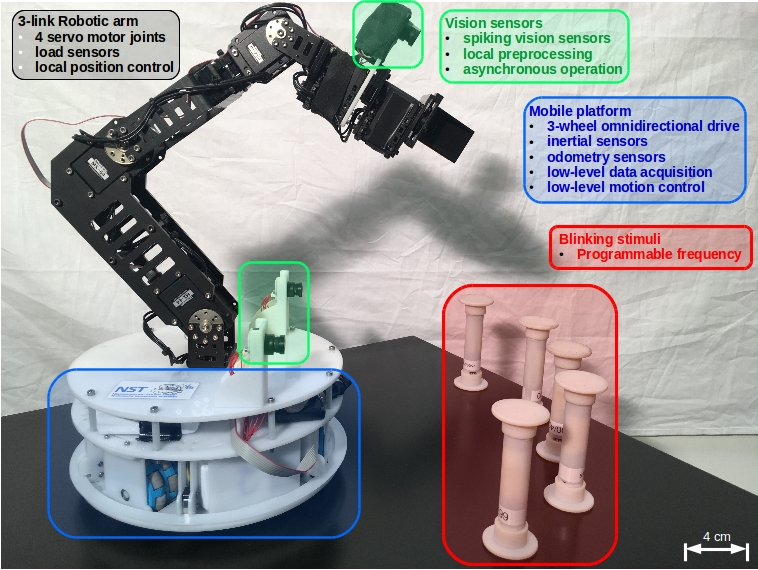
\includegraphics[width=0.8\linewidth]{imgs/omniarmbot.png}
    \caption{Robotic platform}
    \label{fig:omniarmbot}
\end{figure}

\subsubsection{Software setup}%
\label{ssubsec:software_setup}

The overall software architecture is based on a modular design allowing the extension of the current sensorimotor capabilities of the robotic platform by adding more sensors and actuators. 
The software architecture is comprised of an embedded sensorimotor platform running on-board the robot and a neurocomputing platform suitable to run on various computing backends like \ac{CPU}, \ac{GPU} and \ac{NPU}, as shown in Figure \ref{fig:neurocomputing_platform}. 
The embedded platform is responsible with the low-level sensory perception, low-level motor control, and the bi-directional communication (i.e., outgoing data streaming and incoming commands) with the neurocomputing platform. 
\begin{figure}[t]
    \centering
    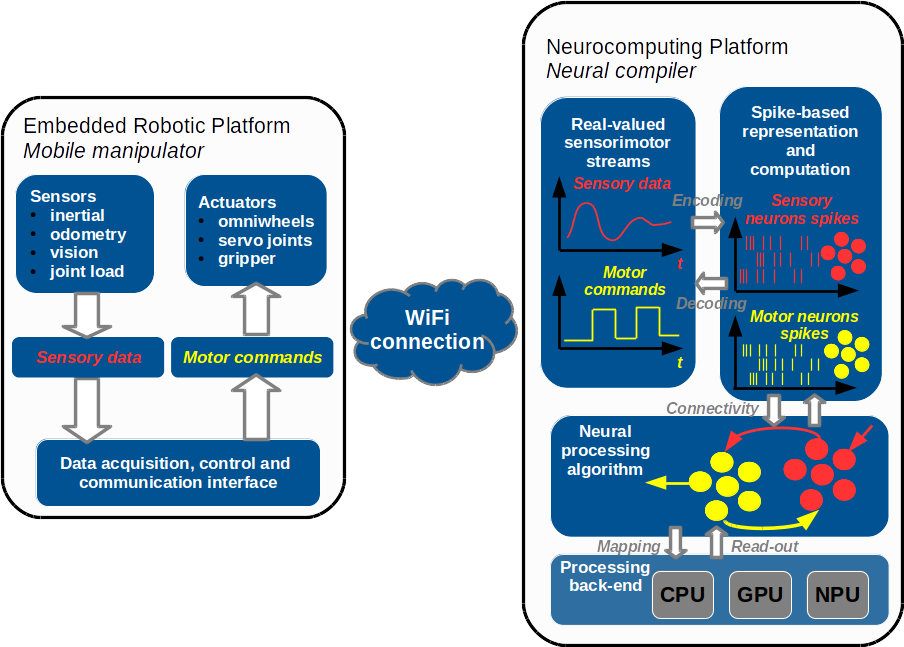
\includegraphics[width=0.8\linewidth]{imgs/neurocomputing_platform.png}
    \caption{Generic architecture: Embedded Robotic Platform and Neurocomputing Platform}
    \label{fig:neurocomputing_platform}
\end{figure}
Decoupling low-level sensorimotor control from the high level behavior, the neurocomputing platform offers a generic interface to implement neurocontrol algorithms. 
This is achieved by separating the representation of the sensorimotor streams, the transformation to be applied on these streams and the actual dynamics of the algorithm. 
Using such a decoupling and a high-level description of the task, the neurocomputing platform acts as a neural compiler. 
Such a neural compiler is able to encode real-world sensorimotor streams in spiking activity over populations of neurons. 
This representation is highly informative and can support efficient computation and learning needed in closed-loop robotic applications where data uncertainty, noise and unstructured environments yield adaptive behavior. 
Supporting intrinsically parallelizable processing mechanisms (i.e., neural networks) the neurocomputing platform can accelerate computation by natively mapping the neural controller on parallel computing hardware.

\subsubsection{Interface infrastructure}%
\label{ssubsec:interface_infrastructure}

The interface between the embedded platform and the neurocomputing platform is designed to abstract the elementary data acquisition and control. 
It encapsulates it in spiking neural activity of neural populations that represent sensory data or generate motor commands as provided by \ac{Nengo}. 
Such an interface allows the neurocomputing platform to natively operate on either real-valued encodings of the sensory data and motor commands or their spike based representations.

\subsection{Neural algorithm development}%
\label{subsec:neural_algorithm_development}

Our overall goal is to develop robotic control systems that are programmable and, at the same time, implemented as neural networks. 
We want them to be programmable so that we can leverage expert knowledge about the steps required to perform a task. 
We want them to be implemented as neural networks partly so that we can make use of energy-efficient neuromorphic hardware, but mostly because neural networks allow for gradual improvement of task performance via learning. 
However, neural networks on their own generally start with zero knowledge (random connection weights) and can often take a long time to learn, or completely fail to learn complex tasks.
What we thus need is a method for taking a complex algorithm (i.e., the program we want to implement) and breaking it down into smaller components. 
Each of those components can then be implemented in a neural network. 
These individual neural networks can then be combined into one large neural network that can perform the entire task. 
This final network can then be implemented in neuromorphic hardware, and it could also be used as the starting point for further learning.
Crucially, it should be noted that we are not trying to implement a perfect version of a task. 
Rather, we want to program a somewhat competent, initial version of a task that could then be further refined using a variety of neural network learning algorithms. 
In particular, \cite{Duan2016} provide a comprehensive survey of Deep Reinforcement Learning algorithms that are suitable for robotic control learning. 
Most of these algorithms are based around adjusting the connection weights of a neural network in order to improve performance on a task, based on occasional “positive” and “negative” reward values. 
Our long-term research goal is to apply these learning systems to the programmed neural networks that we describe in this section.

\paragraph{Network composition}%
\label{par:network_composition}


\begin{figure}
    \centering
    \resizebox{.9\textwidth}{!}{%
        \subfloat[\label{subfig:combined_net} Combined network.]{
        \begin{tikzpicture}[%
        auto,
        multilayer,
        ]
        \Vertices{data/net_1_vertices.csv}
        \Edges{data/net_1_edges.csv}
        \draw (0.5,0)--(0.5,0) node[below]{$y$};
        \draw (4,-2.5)--(4,-2.5) node[above]{$y=f(x)$};
        \draw (0.5,-5)--(0.5,-5) node[below]{$x$};
        \draw (-2.5,-5)--(-2.5,-5) node[below]{$w$};
        \draw (-4,-2.5)--(-4,-2.5) node[below]{$z=g(w)$};
        \draw (-2.5,0)--(-2.5,0) node[below]{$z$};
        \draw (-0.5,5)--(-0.5,5) node[below]{$m$};
        \draw (-2,2.5)--(-2,2.5) node[below]{$m=h(y,z)$};
        \draw (-4.5,0)--(-4.5,0) node[below]{$m=h(f(x),g(w))$};
        \end{tikzpicture}}\qquad
    \subfloat[\label{subfig:direct_net} Direct network.]{
    \begin{tikzpicture}
        \Vertices{data/net_2_vertices.csv}
        \Edges{data/net_2_edges.csv}
        \draw (-2.5,0.5)--(-2.5,0.5) node[below]{$x$};
        \draw (-2.5,-2.5)--(-2.5,-2.5) node[below]{$w$};
        \draw (4.05,0.25)--(4.05,0.25) node[below]{$m$};
        \draw (1.25,-3.25)--(1.25,-3.25) node[below]{$m=h(f(x),g(w))$};
    \end{tikzpicture}}
}
    \caption{Schematic visualization of two neural networks computing a complex function $m=h(f(x), g(w))$:
~\protect\subref{subfig:combined_net} shows a combined network computing $m=h(f(x),g(w))$ while the network in~\protect\subref{subfig:direct_net} computes the function directly.
}
\end{figure}

In order to build larger systems with complex algorithms, we can combine multiple neural networks together.
For example, Figure \ref{subfig:combined_net} shows a system where we not only have $y=f(x)$, but we also have $z=g(w)$, and our final output is a function of the outputs of both of the other two networks, $m=h(y, z)$.
By creating networks to compute these intermediate functions and then combining them together, we can implement complex computations. 
One crucial question, however, is what advantage do we get by breaking this complex function down into smaller, simpler functions. 
After all, it would have been possible to just make one single network that directly approximates the desired function.
The primary reason not to combine functions together is that of scaling. 
As algorithms become more complex, it becomes harder and harder for neural networks to approximate them. 
The traditional solutions are to either increase the number of neurons in the middle layer, or to add more layers. 
Both of these approaches make it harder for the learning algorithms to find the connection weights that best approximate the function, and make the network require more neurons, and thus more computational resources are needed.
Importantly, one can think of Figure \ref{subfig:combined_net} as the result of starting with Figure \ref{subfig:direct_net}, adding in more hidden layers, and adjusting the connectivity. 
In other words, by building a complex network out of smaller networks, we are imposing structure on the network. 
We are specifically indicating that $y$ and $z$ are useful intermediate results that the network should find as an intermediate step before computing $m$. 
If we, as programmers, are correct in our decisions about this intermediate structure, then we can greatly simplify the process of creating these networks.

Given these tools, we can use \ac{Nengo} to automatically construct large neural networks for us. 
In order to do this, we have to take our desired algorithm and break it into small parts, each of which is a function computed on an input vector or a differential equation.

\subsection{Neural task implementation}%
\label{subsec:neural_task_implementation}

Even the simplest behaviors are exploiting relations (i.e., functions) between sensory streams and motor commands. 
In order to design a neural controller able to adaptively switch control policies it is natural to extract such functions in a reliable way, given the variability and uncertainty in the sensorimotor streams. 
The relatively complex and nonlinear interactions among the sensors on the robot and it’s actuators, makes the derivation of analytical forms of such functions hard. 
Alleviating the need for such precise and task-dependent modeling, neural networks are able to approximate such functions just from observations of the available sensorimotor streams. 
Moreover, using learning mechanisms, such systems can ultimately autonomously extract such functions from the data. 
In general, adaptive behavior is regarded as autonomous when the actions performed by the agent result from the interaction between its internal dynamics and the environment. 
Following such a perspective, our system is able to incrementally build up complex behaviors by superimposing more simple, basic behaviors.

In the current instantiation of our framework, we want to solve a non-trivial mobile manipulation task. 
Using our mobile platform the task is to manipulate objects with LED stimuli blinking at different frequencies to bring them in order. 
More precisely, the task can be seen as a grasp and sort task, in which the robot will select a certain control policy depending on the current sensory streams (mainly visual input) to find the misplaced stimulus and place it in the correct location. 
Action selection is performed using a model of a biologically plausible neural circuit, namely the Basal Ganglia. 
The Basal Ganglia, according to \cite{Stewart2010}, is an action selector that chooses whatever action has the best "salience" or "goodness". 
Selection is done on the basis of a context dependent utility signal for each possible action. 
Actions that are inappropriate for the current context may have low utility, and the task of the Basal Ganglia is to select the action that currently has the highest utility value.
The Basal Ganglia will choose between the four possible behavior stacks: Grab, Hold And Move Side, Put Down or Finish.
We design our control network by defining a set of intermediate-level networks, namely Grab, Hold And Move Side, Put Down and Finish that are composed of various different low-level behaviors, and then we create a high-level network whose outputs activate and deactivate the low-level networks. 
To accomplish this, each of the low-level networks will have an input $a$ which indicates its level of activation. 
If $a$ is $0$ then the output from that network should be $0$, and if $a$ is $1$ then it should perform its basic activity. 
It should be noted that this sort of control system design is strongly reminiscent of the classic subsumption architecture \cite{Brooks1986}.
For each of these behaviors, we used \ac{Nengo} to take the functions provided, generate input and output training data, use that data to generate individual neural networks.

\subsubsection{Perception and motor-control: low-level reflex behaviors}%
\label{ssubsec:perception_and_motor_control_low_level_reflex_behaviors}

\paragraph{Orient Left/Right using all cameras}
This behavior uses the $x$-position location of the target in all three camera views to control the rotation of the robot. 
If the object is on the left, it turns left, and if it is on the right, it turns right. 
This should cause the robot to turn to face the object. If it can not see the object, it does nothing. 
If the object can not be seen by a particular camera, it does not contribute.

\paragraph{Orient Left/Right Using Arm Camera Only} 
This behavior is similar to the previous one, but only uses the arm camera. 
This is meant to be used when the arm camera has a good view of the target, allowing for a more fine-grained close-up control.

\paragraph{Move Forward/Backward to Grasping Distance} 
\label{orientFB}
Here, we use the binocular disparity to the object to control whether we should move forward or backward. 
This behavior will output $0$ if the object is not mostly in front of the robot (as computed by averaging the $x$ positions in the left and right camera). 
If it is in front of the robot, then we move forward or backward to achieve the desired disparity (hard-coded to be $0.8$).

\paragraph{Move arm to grasping position} 
\label{grasppos}
This behavior simply moves the arm from its resting position to a position suitable for grasping.

\paragraph{Move Backwards} 
\label{moveback}
This simply moves the robot base backwards.

\paragraph{Close grip} 
\label{grip}
This simply closes the gripper.

\paragraph{Move sideways} 
\label{moveside}
This behavior moves the robot base sideways towards a goal position and rotates the base to keep the goal position in the middle of the field of view of the robot. 
We make use of the target positions of the neighboring objects (cf. \emph{Out of Order} Network), where the middle between them is the goal position of this behavior.

\paragraph{Move arm to put-down position} 
\label{putdownpos}
This behavior simply moves the arm from its holding position to a position suitable for putting down the object again.

\subsubsection{Reasoning: higher-level, cognitive behaviors}%
\label{ssubsec:reasoning_higher_level_cognitive_behaviors}

\paragraph{Out of Order Network} 
\label{outoforder}

\begin{figure}[t]
    \centering
    \resizebox{.9\textwidth}{!}{%
        \subfloat[\label{subfig:omni_bot_out_of_order_net}]{%
            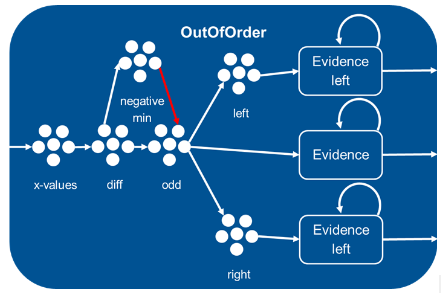
\includegraphics[height=3cm]{imgs/omni_bot_out_of_order_net.png}
        }
        \subfloat[\label{subfig:omni_bot_grab_net}]{%
            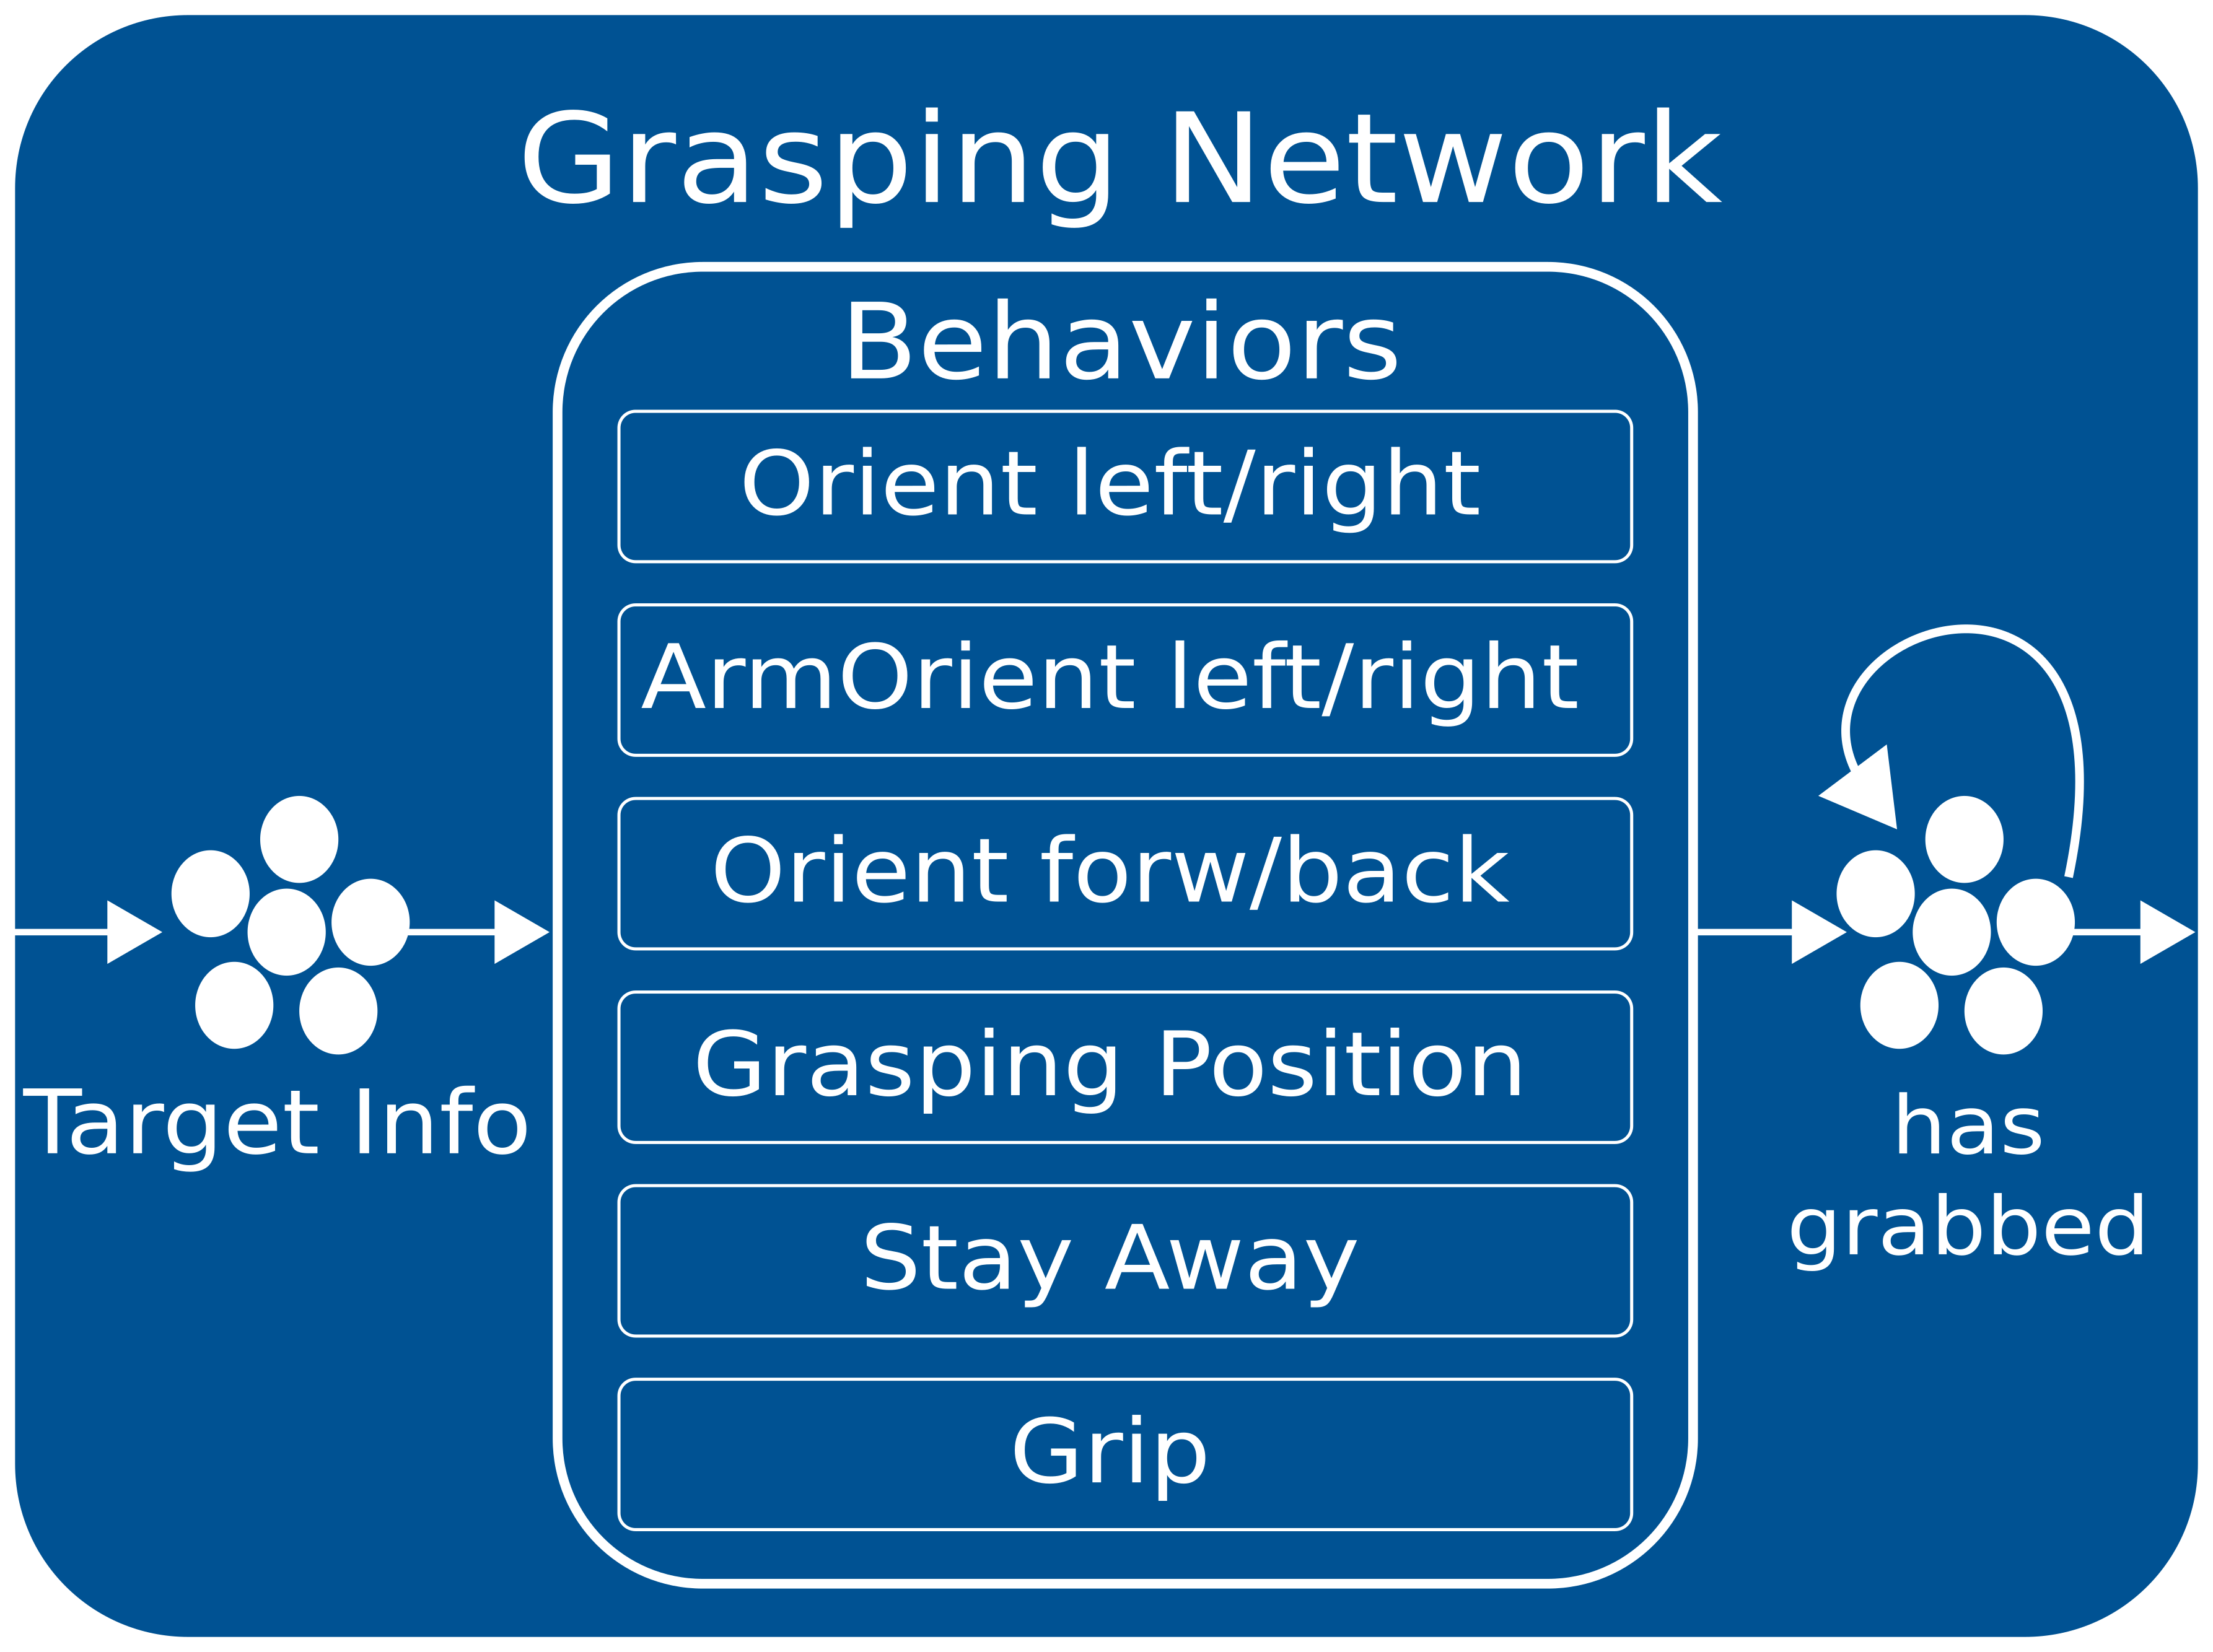
\includegraphics[height=3cm]{imgs/omni_bot_grab_net.png}
        }
    }
    \caption{Schematic visualization of two sub-networks of our model with sets of white circles indicating neural populations while boxes depict sub-networks.
       ~\protect\subref{subfig:omni_bot_out_of_order_net} shows the \emph{Out of Order} network, which detects if one frequency does not fit the assumed order as target and keeps this object’s information in a memory.
~\protect\subref{subfig:omni_bot_grab_net} illustrates the \emph{TaskGrab} network, which finds an object and grabs it.
}
    \label{fig:omni_bot_nets}
\end{figure}

This network computes the object to manipulate and serves as basis for all following behaviors built on top of it. 
Assuming the objects' blinking frequencies are given in descending order, this network detects if one frequency does not fit the assumed order, indicates the corresponding object as target and keeps this object's information in a memory. 
Furthermore, the network detects those frequencies, which should be the neighbors of our detected target if in correct order and keeps their information in a memory as well.
Figure \ref{subfig:omni_bot_out_of_order_net} gives a schematic visualization of the network and its individual components.
The $x$-values ensemble encodes $x$-positions of stimuli in \ac{DVS}-image, the diff ensemble encodes pairwise differences between $x$-positions, the negative-min ensemble indicates if the minimal difference is negative, odd encodes the frequency, which is out of order (inhibited by negative min when all differences are positive), the evidence networks integrate evidence for the target object and the neighbor frequencies if in correct order.
Figure \ref{subfig:omni_bot_out_of_order_net_behavior} shows an example of actual \ac{DVS} input data from the embedded tracking algorithm as well as the decoded output of the network’s sub-components activity: during the first \SI{5}{\second} the stimuli are in correct descending order from left to right in the \ac{DVS}-image (first plot in the left column of Fig. \ref{subfig:omni_bot_out_of_order_net_behavior}), so the minimum pairwise difference is non-negative ( second and third
plots in the left column of Fig. \ref{subfig:omni_bot_out_of_order_net_behavior}). 
In the interval \SIrange{5}{15}{\second}, the \SI{250}{\hertz} stimulus is put between the \SI{150}{\hertz} and \SI{200}{\hertz} stimuli, so now the sequence is out of order and the \SI{250}{\hertz} frequency is detected by the odd ensemble (last row in the left column of Fig. \ref{subfig:omni_bot_out_of_order_net_behavior}) while the evidence networks integrate accordingly (second to last row in the right column of Fig. \ref{subfig:omni_bot_out_of_order_net_behavior}). 
Starting from around \SI{15}{\second} the \SI{250}{\hertz} and \SI{350}{\hertz} stimuli are interchanged and the network's outputs change accordingly (left column of Fig. \ref{subfig:omni_bot_out_of_order_net_behavior}).
However, the evidence networks - as desired - still keep the information about the old target until a forget mechanism (first row of the right column in Fig. \ref{subfig:omni_bot_out_of_order_net_behavior}) is triggered in the interval \SIrange{20}{25}{\second} allowing the evidence networks to recover for new input (right column of Fig. \ref{subfig:omni_bot_out_of_order_net_behavior}).

\paragraph{Perform Grasping Action} 
\label{grasp}

\begin{figure}[th!]
    \centering
    \subfloat[\label{subfig:omni_bot_out_of_order_net_behavior}Decoded output of the \emph{Out of Order} network's neural components based on \ac{DVS} input data from embedded tracking]{%
        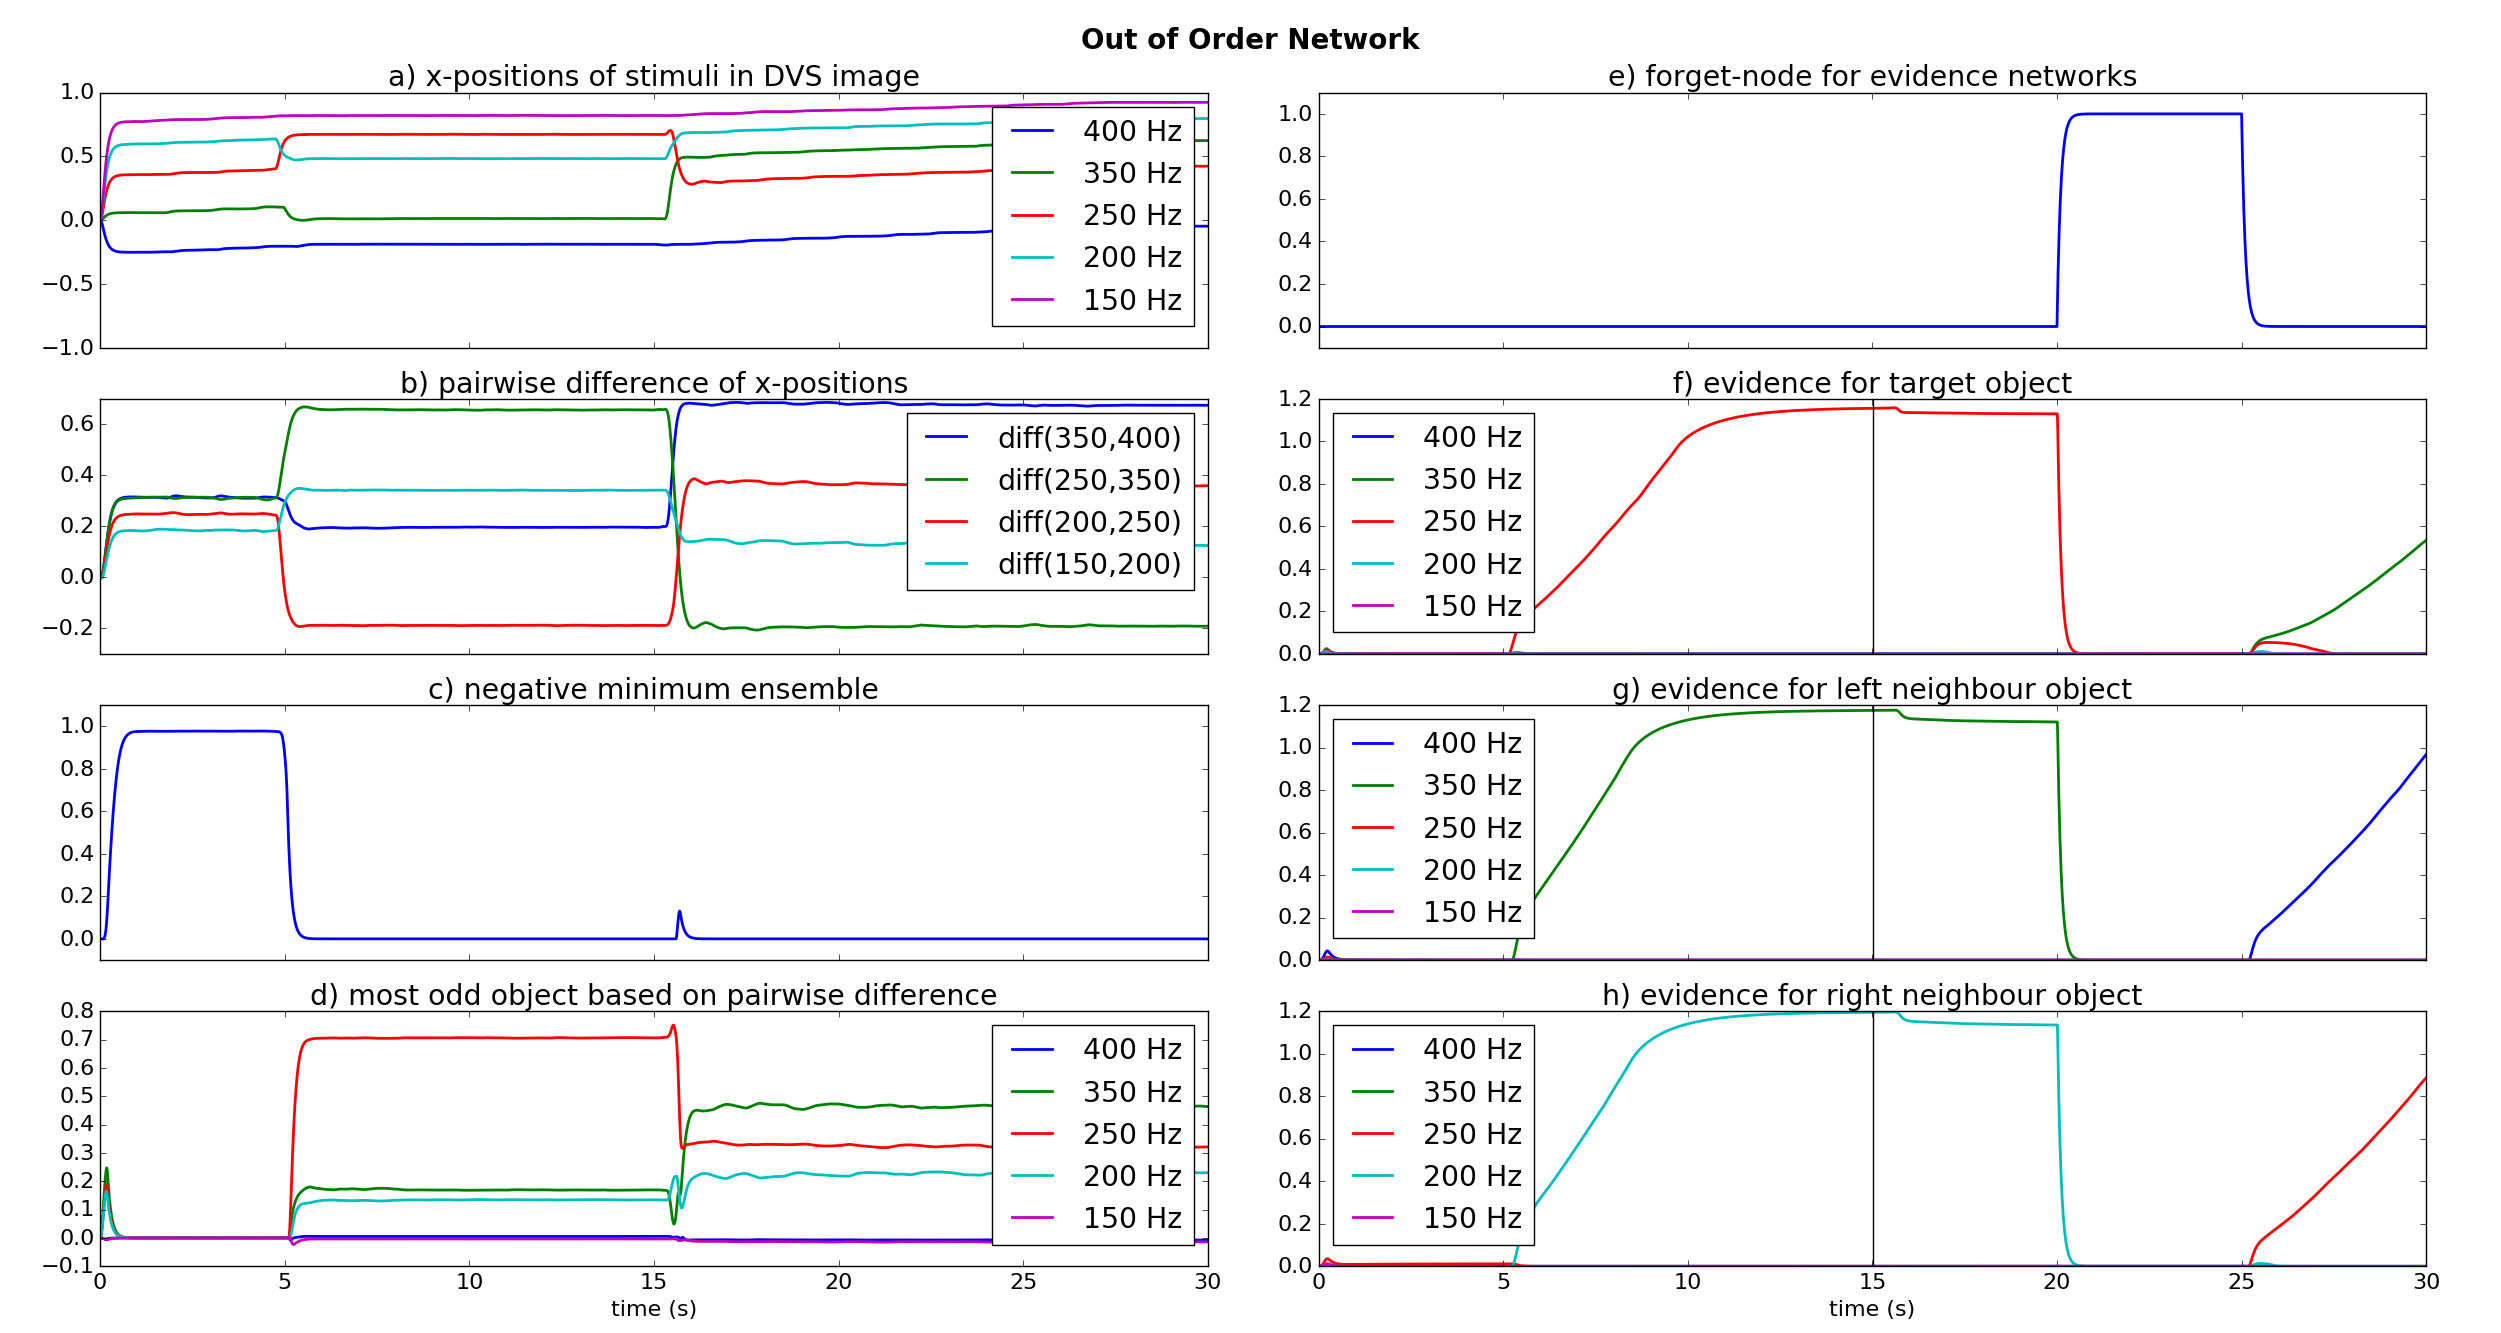
\includegraphics[width=0.9\linewidth]{imgs/omni_bot_out_of_order_net_behavior.png}
    }\\
    \subfloat[\label{subfig:omni_bot_grab_net_behavior}Decoded output of the \emph{Grab} network's neural components]{%
        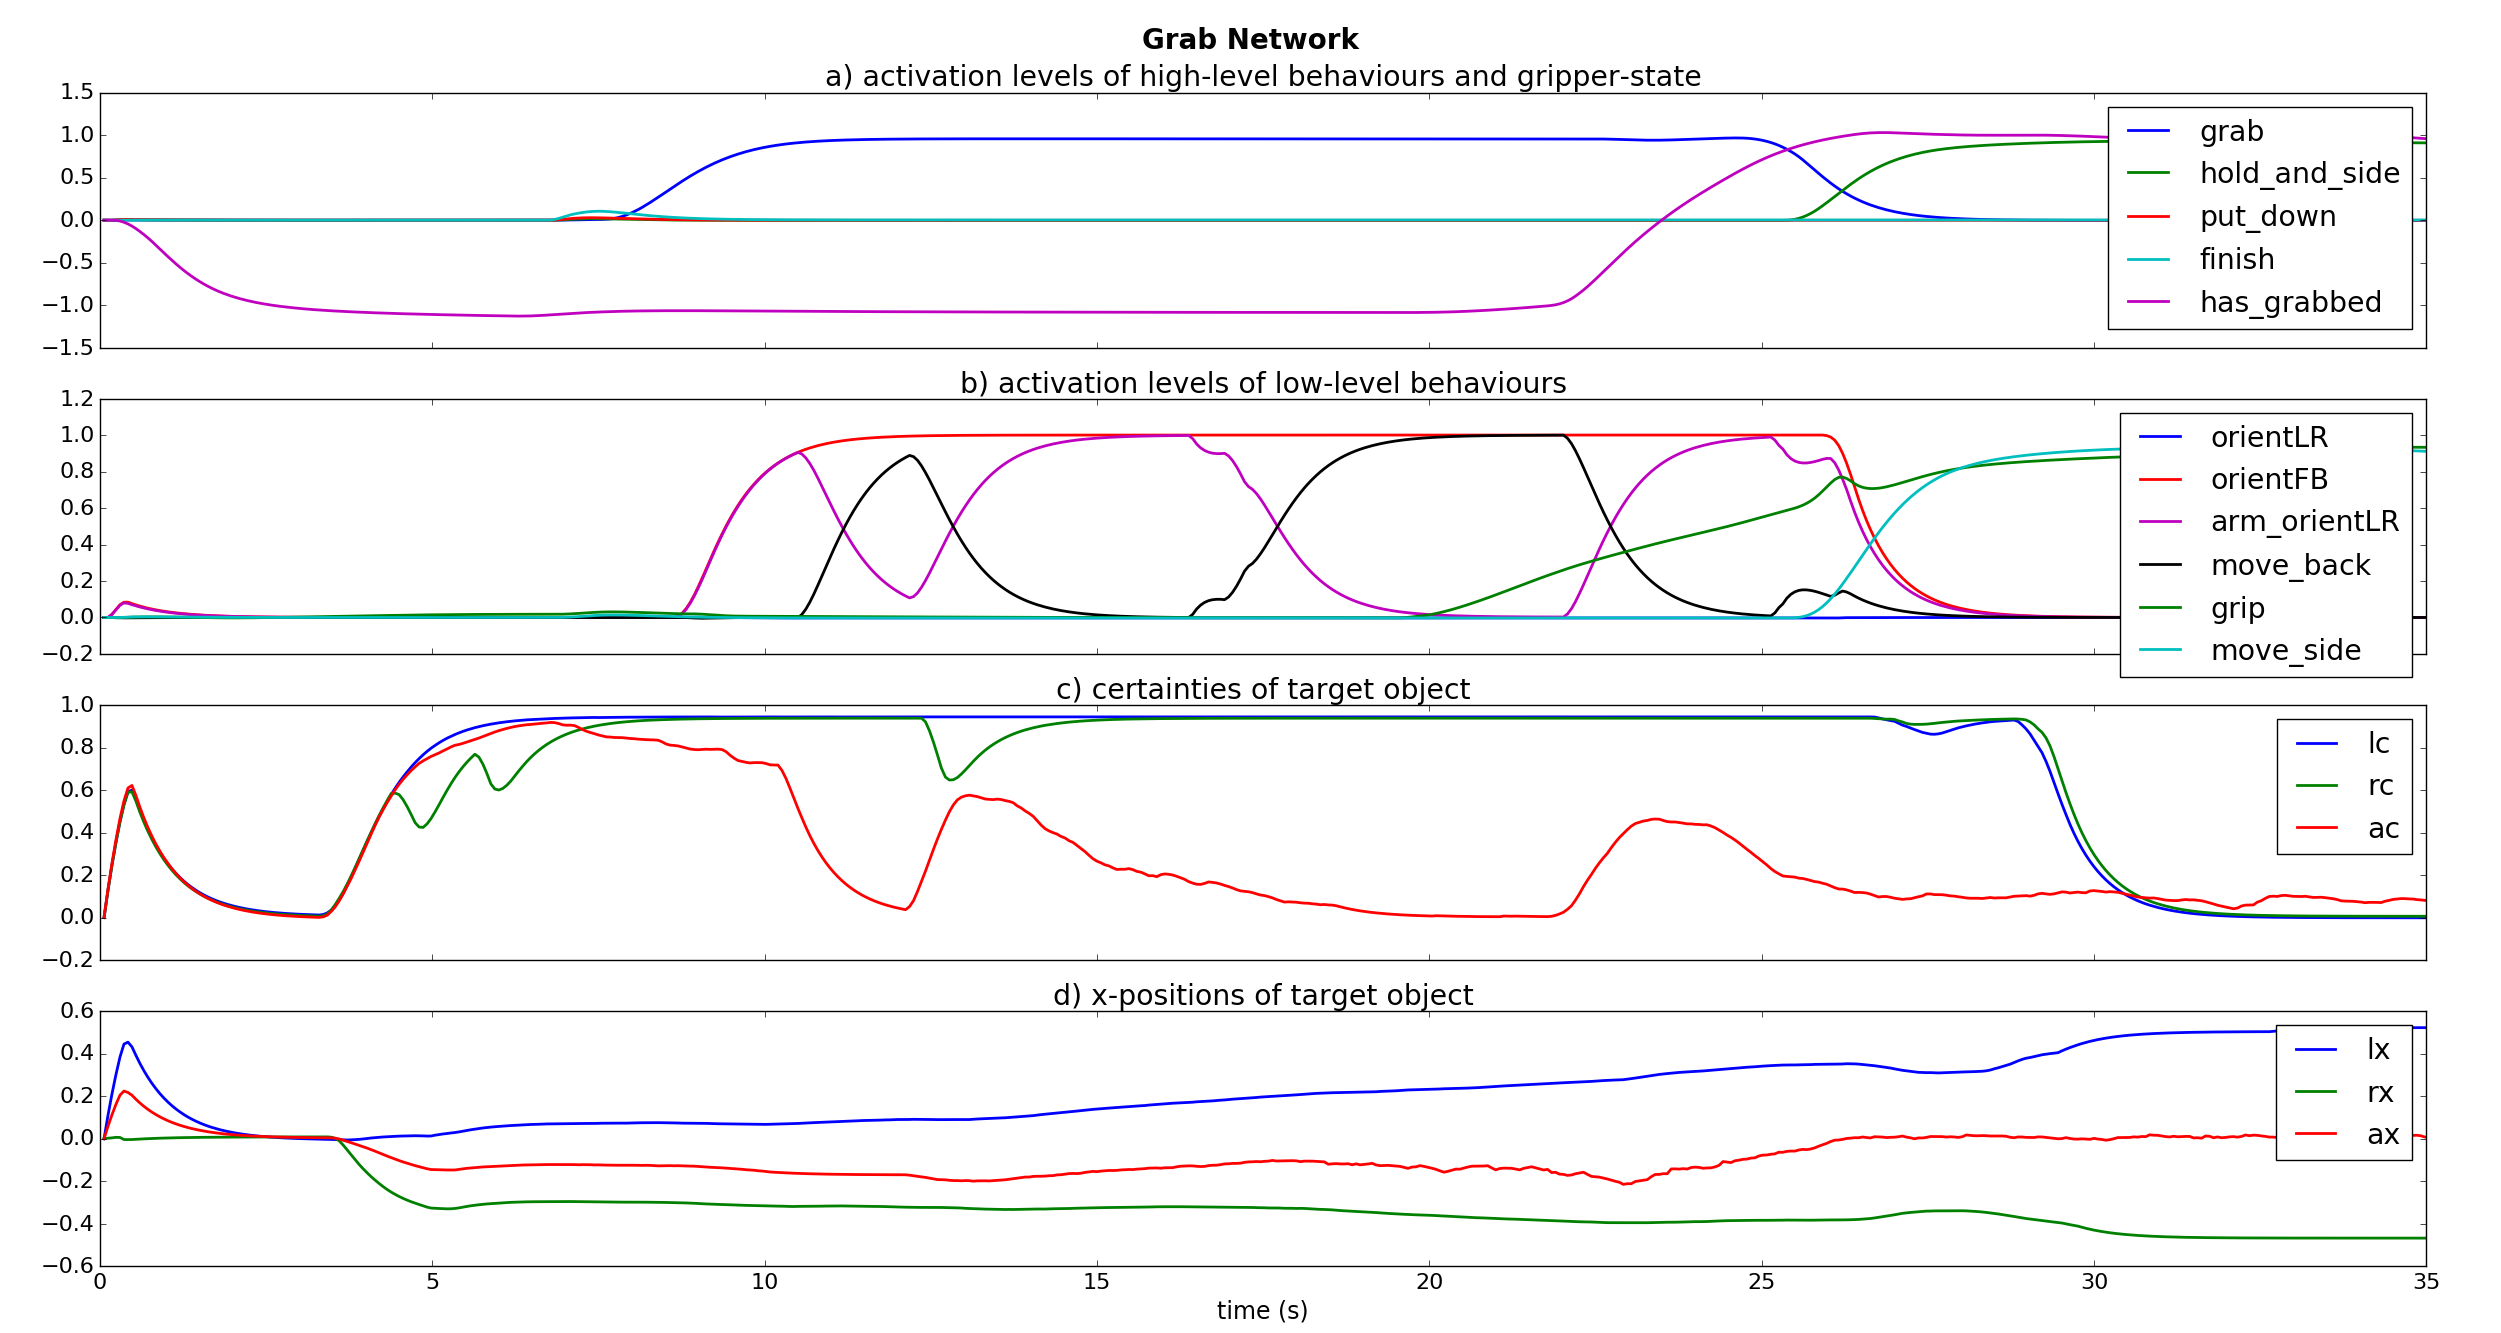
\includegraphics[width=0.9\linewidth]{imgs/omni_bot_grab_net_behavior.png}
    }
    \caption{Illustration of the \emph{Out of Order} and \emph{Grab} networks neural populations decoded output.}
    \label{fig:omni_bot_nets_results}
\end{figure}

This is a high-level behavior that uses the low-level behaviors.
The idea here is to find the object. If the robot can't see it in both cameras, then it backs up until it can. 
Move forward and backward until the robot is at the right distance. 
If the robot can see the object with the arm camera, then it uses the arm camera for orientation, otherwise it uses all three. 
Also, if the robot can't see the object with the arm camera, then it backs up. 
Note that the \emph{MoveBack} behavior and the \emph{Orientation} behaviors both move the robot forward and backward, so when they are both active the robot will end up achieving a position farther away from the object than when just \emph{Orientation} behavior is active (the motor commands are summed). 
This positions the robot such that it can move forward and grab the object. 
Finally, if the robot is at the correct distance from the object (as measured by binocular disparity), and it's right in front of it, then it closes the gripper. 
This combination of actions serves to successfully grab the object. 
Figure \ref{subfig:omni_bot_grab_net} gives a schematic visualization of this network.
The \emph{TargetInfo} ensemble encodes sensory information ($x$- and $y$-position in the image, as well as radius and track-certainty for each \ac{DVS}) of the target object (coming from the \emph{evidence} sub-network in the out of order network), which serves as input for the low-level behaviors.
The \emph{has-grabbed} ensemble keeps the information once the object was grabbed in memory to indicate this task finished successfully.
Figure \ref{subfig:omni_bot_grab_net_behavior} shows the activation levels of the high- and low-level behaviors (first two rows of Fig. \ref{subfig:omni_bot_grab_net_behavior}) as well as the sensory information the behaviors make use of, namely tracking certainty and disparity and $x$-position of the target object in the arm retina (last two rows in Fig. \ref{subfig:omni_bot_grab_net_behavior}). 

\paragraph{Hold Object and Move To Goal Position} 
\label{holdmoveside}
This behavior combines holding an object by keeping the gripper closed while moving to the goal position at the same time. 
Here, we make use of the stored information about the target object`s neighbors to calculate the goal position. 
Therefore, we use the mean value of the lateral positions of the left neighbor in the left base camera and the right neighbor in the right base camera as an estimation of the middle between the neighbor objects, which is where we want to place our target object. 
This value is used to control sideways and rotation motion of the base to navigate the robot to the correct position for putting down the target object (see Fig. \ref{subfig:omni_bot_hold_and_move_behavior} in the interval from \SIrange{28}{37}{\second}). 
Figure \ref{subfig:omni_bot_hold_and_move_net} gives a schematic visualization of this network. 
The Left/Right \emph{TargetInfo} ensembles encode sensory information ($x$- and $y$-position in the image, as well as radius and track-certainty for each \ac{DVS}) of the neighbor objects (coming from the left/right evidence networks in the out of order network), which serves as input for the low-level behaviors.
The \emph{MoveSideways} behavior uses the mean value of the lateral positions of the left and right neighbor in the left and right base camera respectively as an estimation of the middle between the neighbor objects and moves the base to this position, while the \emph{Grip} behavior keeps the gripper closed.
The \emph{Reached position} ensemble serves as a memory integrating evidence once the goal position is reached to indicate that this sub-tasks finished successfully.
Figure \ref{subfig:omni_bot_grab_and_sort_net_behavior} shows the activation levels of the high- and low-level behaviors.

\begin{figure}[t]
    \centering
    \resizebox{.9\textwidth}{!}{%
        \subfloat[\label{subfig:omni_bot_hold_and_move_net}]{%
            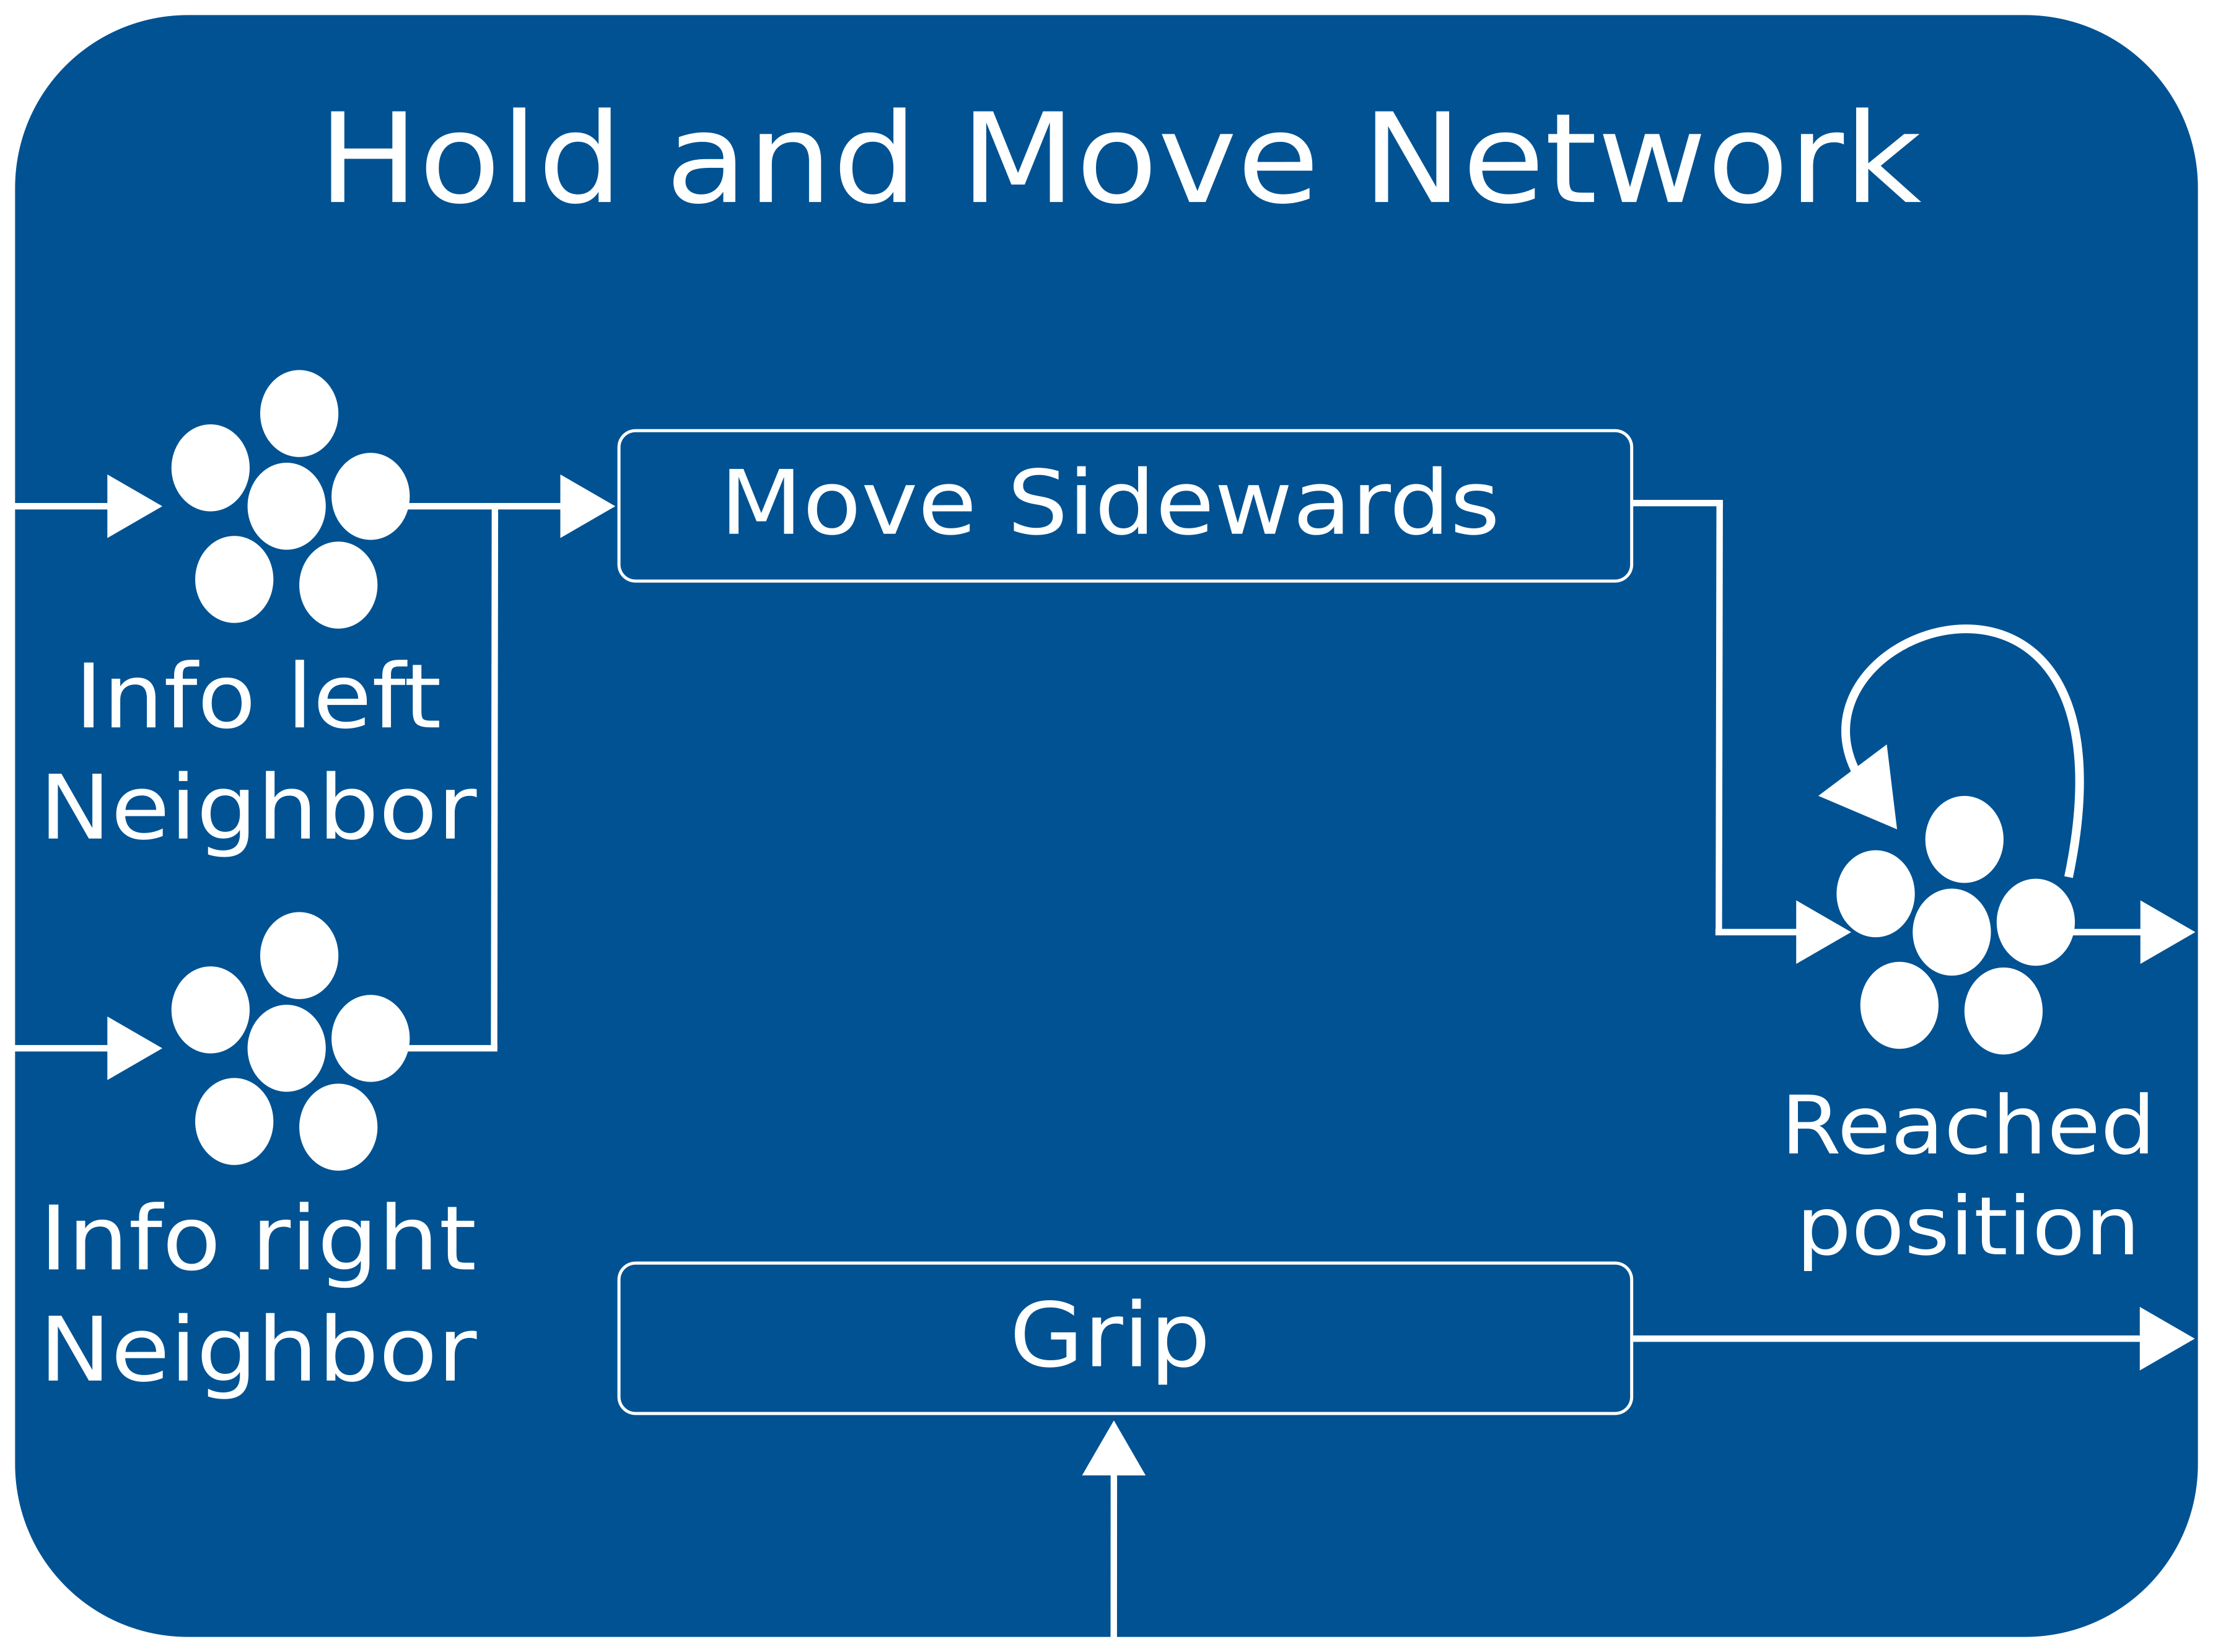
\includegraphics[height=3cm]{imgs/omni_bot_hold_and_move_net.png}
        }
        \subfloat[\label{subfig:omni_bot_grab_and_sort_net}]{%
            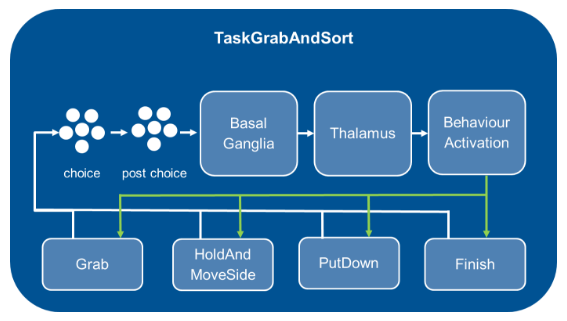
\includegraphics[height=3cm]{imgs/omni_bot_grab_and_sort_net.png}
        }
    }
    \caption{Schematic visualization of two networks of our model with sets of white circles indicating neural populations while boxes depict sub-networks.
       ~\protect\subref{subfig:omni_bot_hold_and_move_net} shows the \emph{HoldAndMove} network, while~\protect\subref{subfig:omni_bot_grab_and_sort_net} illustrates the complete Sorting network.
The boxes in the lower part visualize the subtask-networks, which are activated by the upper network chain for action selection incorporating the Basal Ganglia and Thalamus networks pre-implemented in \ac{Nengo}.
    }
    \label{fig:omni_bot_nets_sort}
\end{figure}

\paragraph{Put Object Down} 
\label{putdown}
This behavior simply moves the arm from its gripping position to a position suitable for releasing an object, while opening the gripper and moving the base slightly backwards at the same time to ensure smooth and safe placement of the target object.

\paragraph{Finish Task} 
\label{finish}

This behavior simply makes the robot base back off from the manipulated objects. 
After stopping the base - implicitly by deactivating all other behaviors - the arm moves to back resting position automatically, which indicates that the whole sequence of tasks is completed.

\paragraph{Perform Sorting Task} 
\label{sort}

\begin{figure}[th!]
    \centering
    \subfloat[\label{subfig:omni_bot_hold_and_move_behavior}Decoded output of the \emph{HoldAndMove} network's neural components]{%
        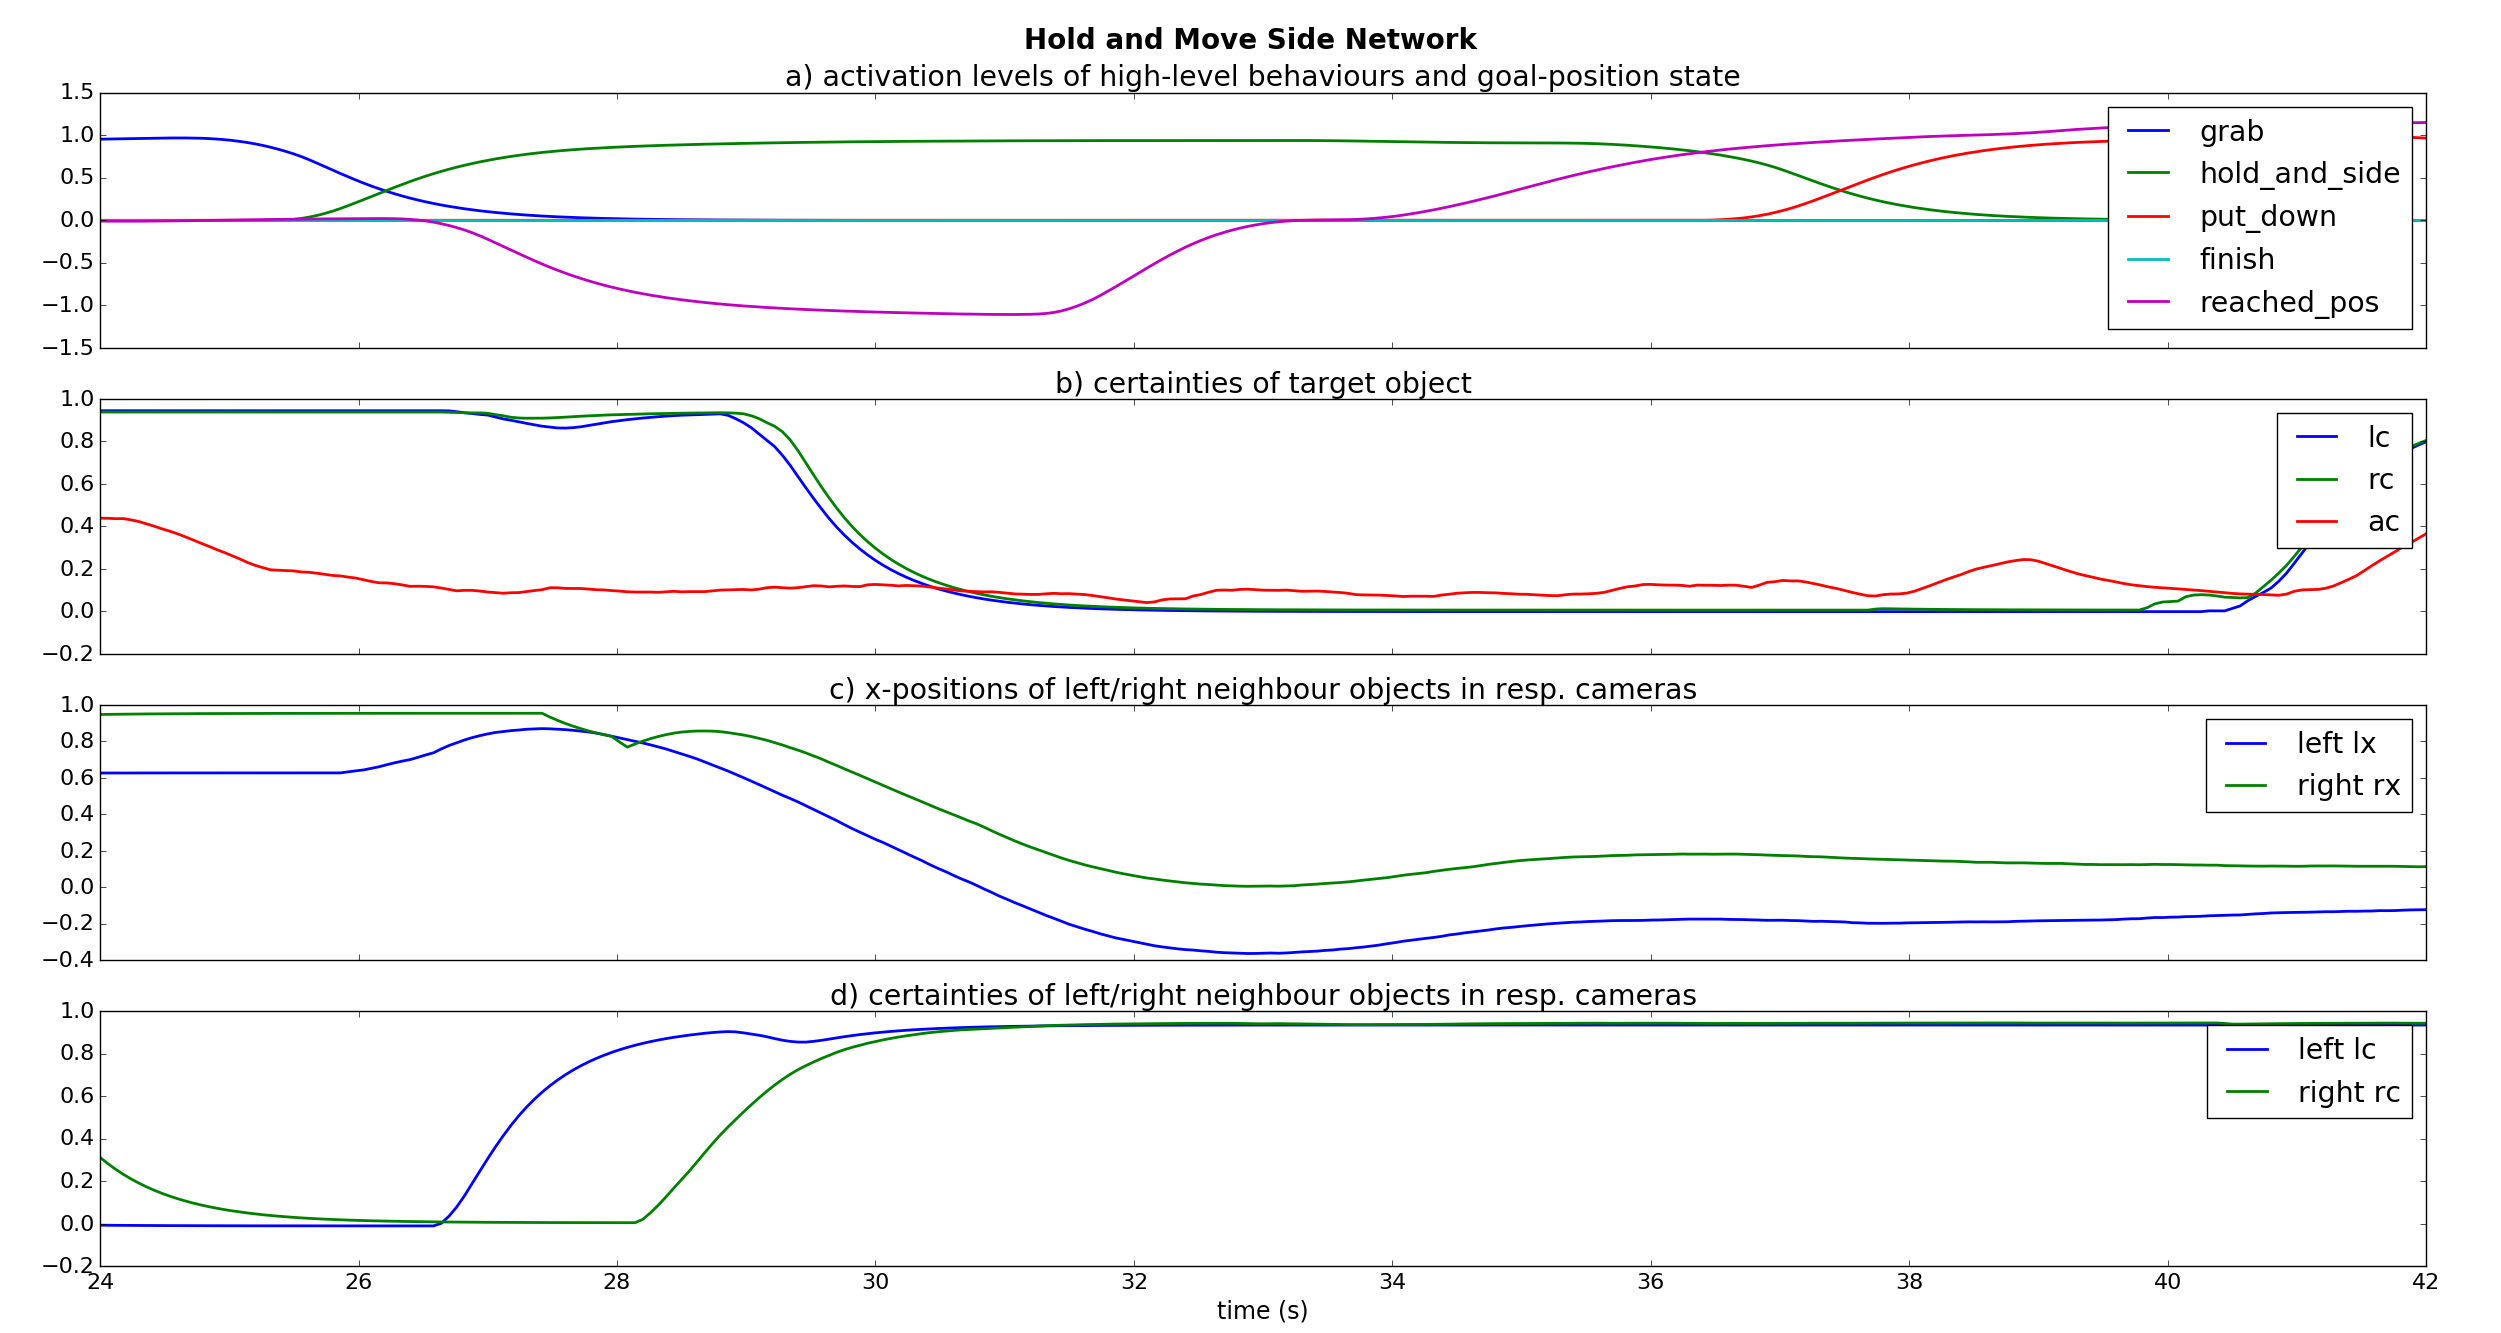
\includegraphics[width=0.9\linewidth]{imgs/omni_bot_hold_and_move_behavior.png}
    }\\
    \subfloat[\label{subfig:omni_bot_grab_and_sort_net_behavior}Decoded output of the \emph{Sorting} network's neural components]{%
        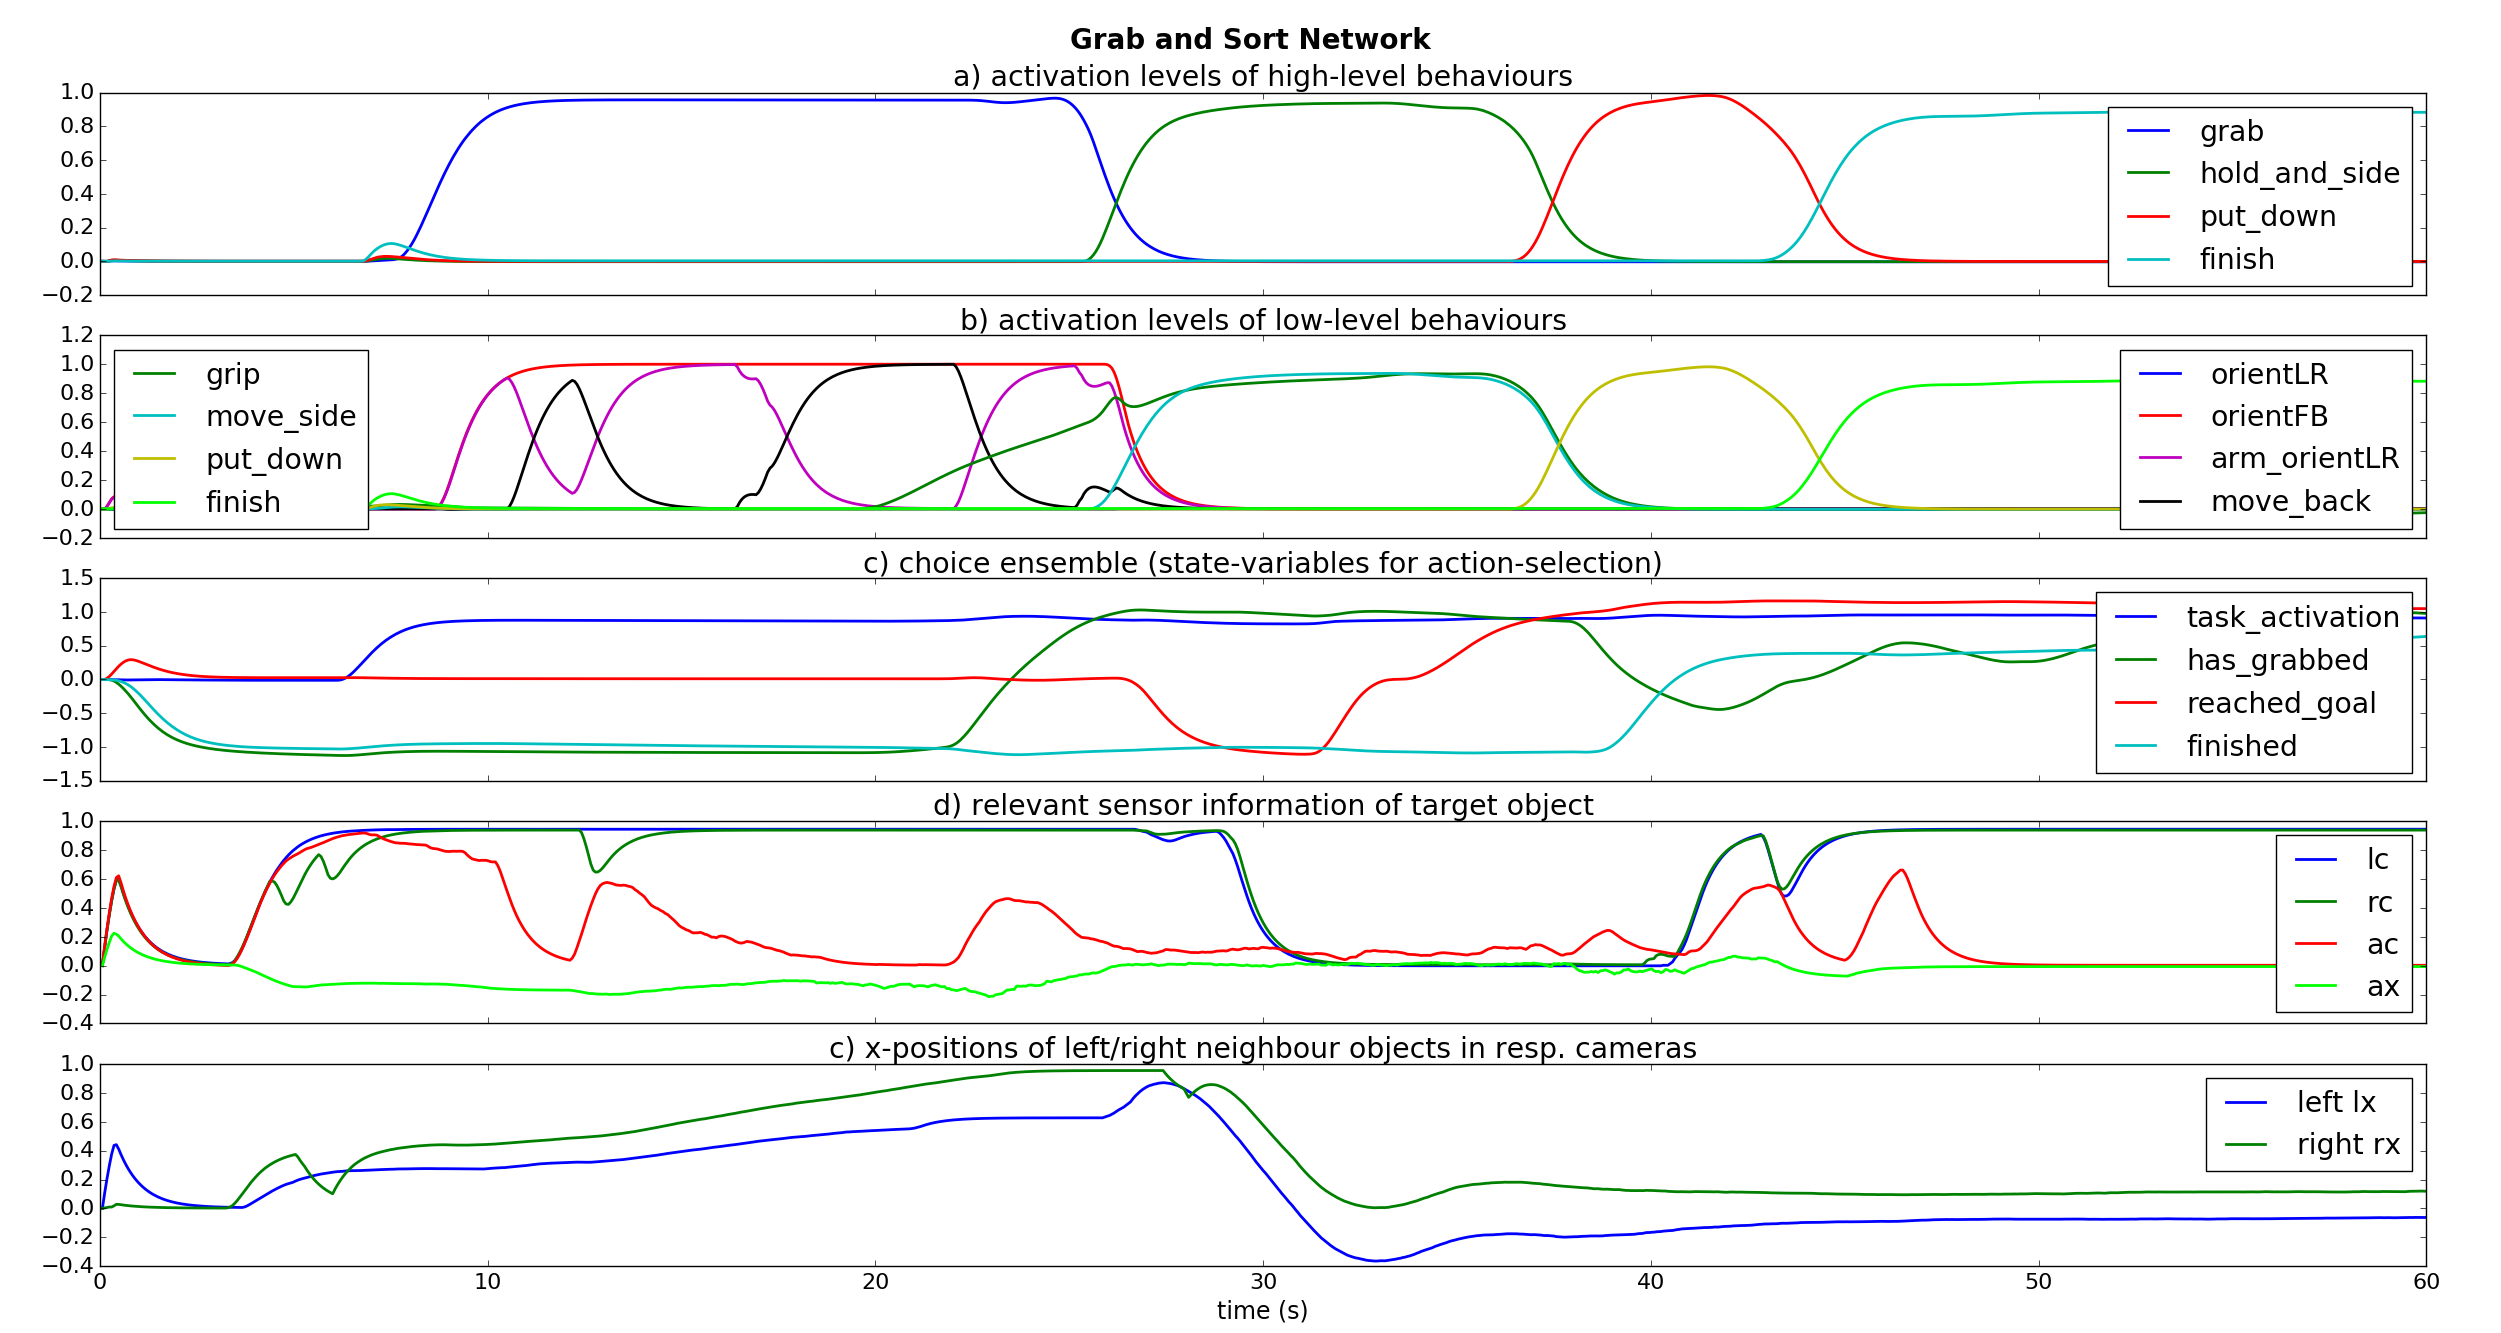
\includegraphics[width=0.9\linewidth]{imgs/omni_bot_grab_and_sort_behav.png}
    }
    \caption{Illustration of the \emph{HoldAndMove} and \emph{Sorting} networks neural populations decoded output.}
    \label{fig:omni_bot_nets_sort_results}
\end{figure}

This is a high-level behavior combining all the other behaviors described so far to complete the whole task of moving the target object to its correct position in the sequence of frequencies. 
To choose the appropriate action to take, we used models of the Basal Ganglia and Thalamus \cite{Stewart2010}, which are available as pre-implemented networks in \ac{Nengo}.
Corresponding to each of the high-level behaviors, we created input values for the Basal Ganglia network to choose from. 
Initially, \emph{Perform Grasping Action} is enabled. 
Once the robot picked up the target object and built up sufficient evidence, the Basal Ganglia network activates the behavior to hold the (target) object and navigate the robot to the goal position. 
As soon as the robot reached its goal position between the neighbor objects and the according network built sufficient evidence, the \emph{PutDown} behavior to put down the target object is activated. 
As soon as this behavior is completed, the whole sequence is wrapped up by activating the \emph{Finish} behavior. 
Figure \ref{subfig:omni_bot_grab_and_sort_net} gives a schematic visualization of the network. 
Figure \ref{fig:omni_bot_example_run} illustrates the most important stages of one example run while Figure \ref{subfig:omni_bot_grab_and_sort_net_behavior} gives a visualization of the decoded output of the network’s components: once the \emph{Out of Order} network detected the target object (roughly the first \SI{5}{\second}), the \emph{Grab} behavior is activated to find and grasp the target object (Fig. \ref{fig:omni_bot_example_run} a-c, Fig. \ref{subfig:omni_bot_grab_and_sort_net_behavior}, t = 8s - 26s). 
The different low-level behaviors for orientation and navigation are enabled based on the certainty and disparity of the tracked stimuli. 
Once the robot grabbed the target object, the \emph{Basal Ganglia} activates the \emph{HoldAndMoveSide} behavior (Fig. \ref{fig:omni_bot_example_run}d-e, Fig. \ref{subfig:omni_bot_grab_and_sort_net_behavior}, t = 26s - 39s). 

The main sensory input in this phase is the $x$-position of the neighbor objects (last row in Fig. \ref{subfig:omni_bot_grab_and_sort_net_behavior}). 
A clear indicator for successful pick-up is the decrease of certainty in the base-retinas (forth row in Fig. \ref{subfig:omni_bot_grab_and_sort_net_behavior}). 
Once the robot reached its goal position between the neighboring objects, the \emph{PutDown} behavior is activated (Fig. \ref{fig:omni_bot_example_run} f-g). 
Finally the whole task is wrapped up by the Finish behavior and all other behaviors are deactivated (Fig. \ref{fig:omni_bot_example_run} h) to put the robot back into resting position.

\begin{figure}[t]
    \centering
    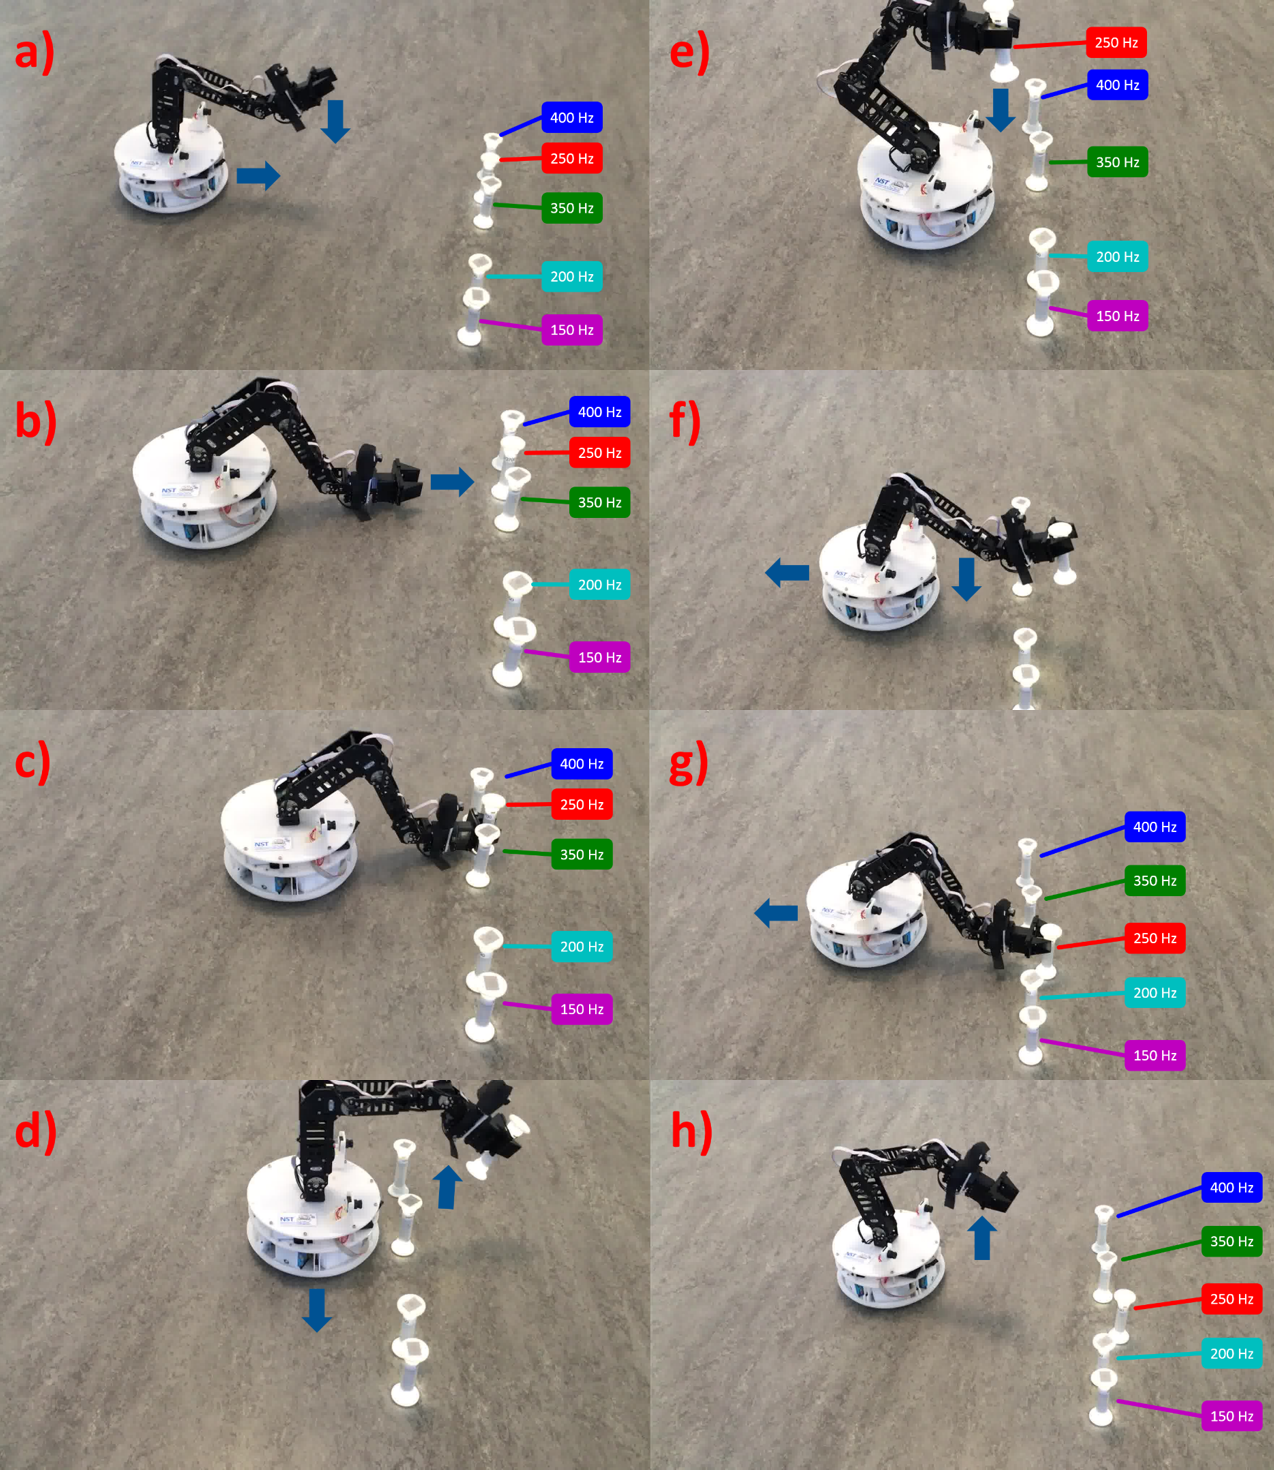
\includegraphics[width=0.8\linewidth]{imgs/omni_bot_example_run.png}
    \caption{Selected stages of an example run of the Grab and Sort Task.}
    \label{fig:omni_bot_example_run}
\end{figure}
\subsection{Summary}%
\label{subsec:summary_mobile_manipulation}

In this section, we have shown a mobile robotic manipulator capable of solving a pick-and-place task, with algorithmic components completely implemented in the framework of \aclp{SNN}. 
This makes our approach not only suitable to expand its functionality with supervised and unsupervised learning methods but also highly scalable. 
The underlying \ac{Nengo}-based neural compiler supports the use of dedicated neuromorphic hardware systems, which allows to run even large-scale neural networks in real-time. 
The possibility to introduce learning will eventually enable such systems to adapt its control policies and decision making to unpredictable changes in the environment. 
Furthermore, the neural implementation is beneficial in terms of allowing to combine networks “hand-programmed” by experts/engineers with learning networks that improve themselves over time with increasing data/experience. 
Here, our ultimate goal is to design systems that are capable of adapting to new task during operation time while at the same time using experience from previous tasks and expert knowledge.

\subsubsection{Limitations}%
\label{ssubsec:limitations}

The current algorithmic implementation has some inherent limitations. 
For now, the network is only able to detect one object not fitting in the sequence of frequencies. 
To overcome this limitation, the Out of Order network \ref{outoforder} could be enhanced to solve the sorting-problem in a neural fashion. 
An intermediate workaround could be to repeat the current simple task and thereby solve the sorting problem incrementally. 
Another obvious limitation of the current implementation is the need for neighbor objects to find the goal position for put-down. 
This makes it impossible to solve the task for those objects blinking at a maximum or a minimum frequency. 
As for the first limitation, the Out of Order network needs to become more sophisticated to detect the goal position in these edge-cases when a border-object needs to be manipulated. 
One possibility could be detect one neighbor and to use the maximum of the pairwise differences as distance estimation for the offset. 
%Another technical improvement focuses on the embedded tracking algorithm. The efficient frameless tracking algorithm has the disadvantage that the arm retina gets over-flooded with events, when the distance to the target object decreases, which can corrupt the grab-task. 

\subsubsection{Outlook}%
\label{ssubsec:outlook}

A long-term goal is to use the current implementation as a starting point for self-improving learning systems. 
As the current implementation is built in the framework of \acrlong{SNN} it naturally supports learning. 
One direction for future research could be to use the current low-level behaviors for initialization and to let the system learn and improve them incrementally by experience. 
For instance, one problem in learning robotic systems such as policy search for motor control \cite{Levine2015}, is the acquisition of sufficiently large training data sets. 
Recording large amounts of training data by repeating one specific task with real robotic systems is time-consuming and often infeasible, while training-data from simulation is usually not realistic enough to capture the complexity of noisy real-world data. 
In these cases, a system which is able to use expert-knowledge for certain (sub-) tasks as a starting point could significantly speed-up the learning process. 
We believe that our current approach is a promising first step for further research in this direction.


\section{Neuromorphic reinforcement learning for vehicle trajectory control}%
\label{sec:neuromorphic_reinforcement_learning_for_vehicle_trajectory_control}

In this section, we propose a neuromorphic system for vehicle control.
Our system is implemented entirely in a spiking neuron substrate using the \ac{Nengo} simulator \cite{Bekolay2014} and is designed to be both distributed and hierarchical.
In a sample instantiation, we train a trajectory selection module using reinforcement learning to investigate the feasibility of a learnable, neuromorphic control system in an automotive context.
This approach has been selected in order to be decoupled from the quality of training data in this first investigation.
We evaluate our approach in \ac{TORCS}, which allows us to generate training data in a safe and controlled simulation environment.
Furthermore, \ac{TORCS} offers an advanced vehicle physics simulation as well as a variety of sensors and actors for interaction \cite{TORCS}.

\subsection{Neuromorphic control architecture}%
\label{subsec:neuromorphic_control_architecture}

\begin{figure}[t!]
\centering
  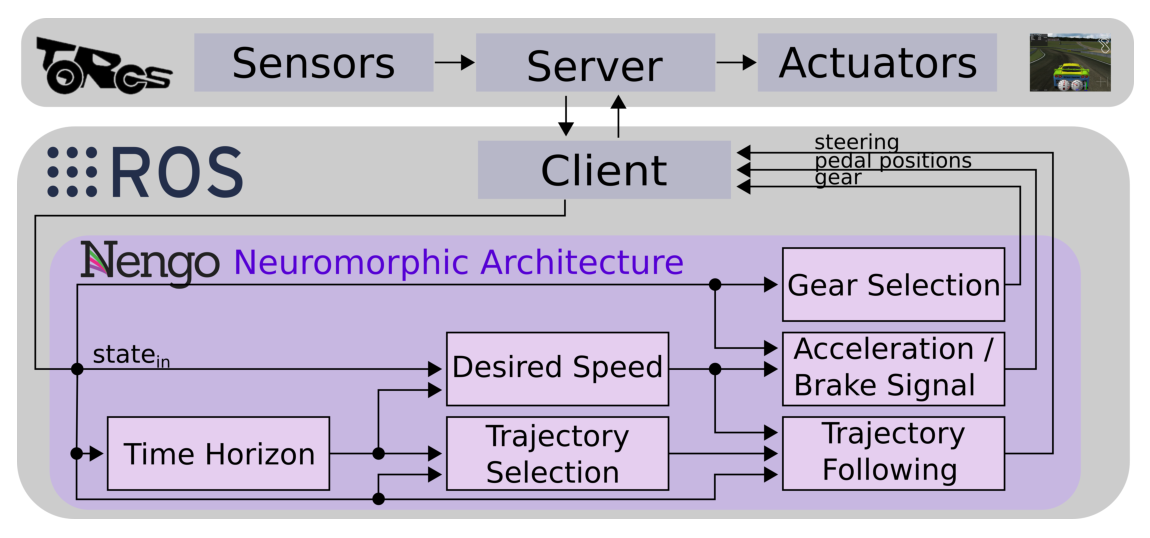
\includegraphics[width=0.95\textwidth]{imgs/Distributed-System-narrow.eps}
\caption{Proposed distributed neuromorphic architecture utilizing individual modules for separate control signal calculation. \label{fig:architecture}}
\end{figure}

The architecture of our proposed system is visualized in Fig.~\ref{fig:architecture}.
Interactions with the \ac{TORCS} environment (for detailed information on the sensor and actuator setup see \cite{Loiacono2010}) are channeled over several \ac{ROS} nodes used for the gateway communication.
For evaluation and training purposes, a controller using the global position and orientation of the vehicle is implemented in \ac{ROS} to determine control signals to follow a given trajectory or the roadways centerline at a fixed speed\footnote{The \ac{TORCS}-to-\ac{ROS} interface can be found at \url{https://github.com/fmirus/torcs_ros}.
The Nengo and \ac{ROS} implementation of the trajectory selection module and the framework that is built upon it can be found at \url{https://github.com/fmirus/torcs_neural_trajectory_ctrl}}.\par

The proposed architecture for a learnable and energy-efficient vehicle control system is a holistic neuromorphic approach for determining steering, gas and brake pedal as well as gear signals.
It is a distributed system in that these signals are calculated separately in different modules.
In addition, it is a hierarchical system as several intermediate values have to be calculated and different modules and subsystems are dependent upon each other.
The modules' vertical alignments within Fig. \ref{fig:architecture} indicate the distinction of three core subsystems, each responsible for one of the control signals (\emph{gear selection}, \emph{breaking/acceleration} and \emph{steering}).
We envision each of these sub-modules to be learnable either by supervised or reinforcement learning.
Some of the depicted modules are heavily dependent on each other and will have to be trained in parallel rather than independently. 

Here, we focus on the \emph{trajectory selection} module to be the only learning module for simplicity.
Therefore, gear selection and acceleration are determined from the engine's rpm and a desired velocity set to a fixed value for now.
The \emph{trajectory following} module determines the control values for steering from the chosen trajectory.
% Implicitly,  \emph{trajectory selection} and \emph{trajectory following} achieve a similar goal to the sweep for a trajectory's lateral and longitudinal characteristics in \cite{Werling2010}.
We envision the \emph{time horizon} module to estimate the time window for the next trajectory to be followed.
Assuming a perfect control algorithm and the desired speed to be the actual speed, this equates to determining the trajectory's end point's longitudinal position.
Accordingly, the \emph{trajectory selection} module is an action selection module for the agent to choose a trajectory type as well as the lateral component of the trajectory's end point from a set of predefined options.

\begin{figure}[t!]
\centering
\subfloat[Simplified visualization of the \ac{SNN} for \textit{trajectory selection}. The yellow ($A$) resp. cyan networks ($B$) implement action selection resp. weight optimization for three exemplary trajectory choices \label{fig:snn}]{
  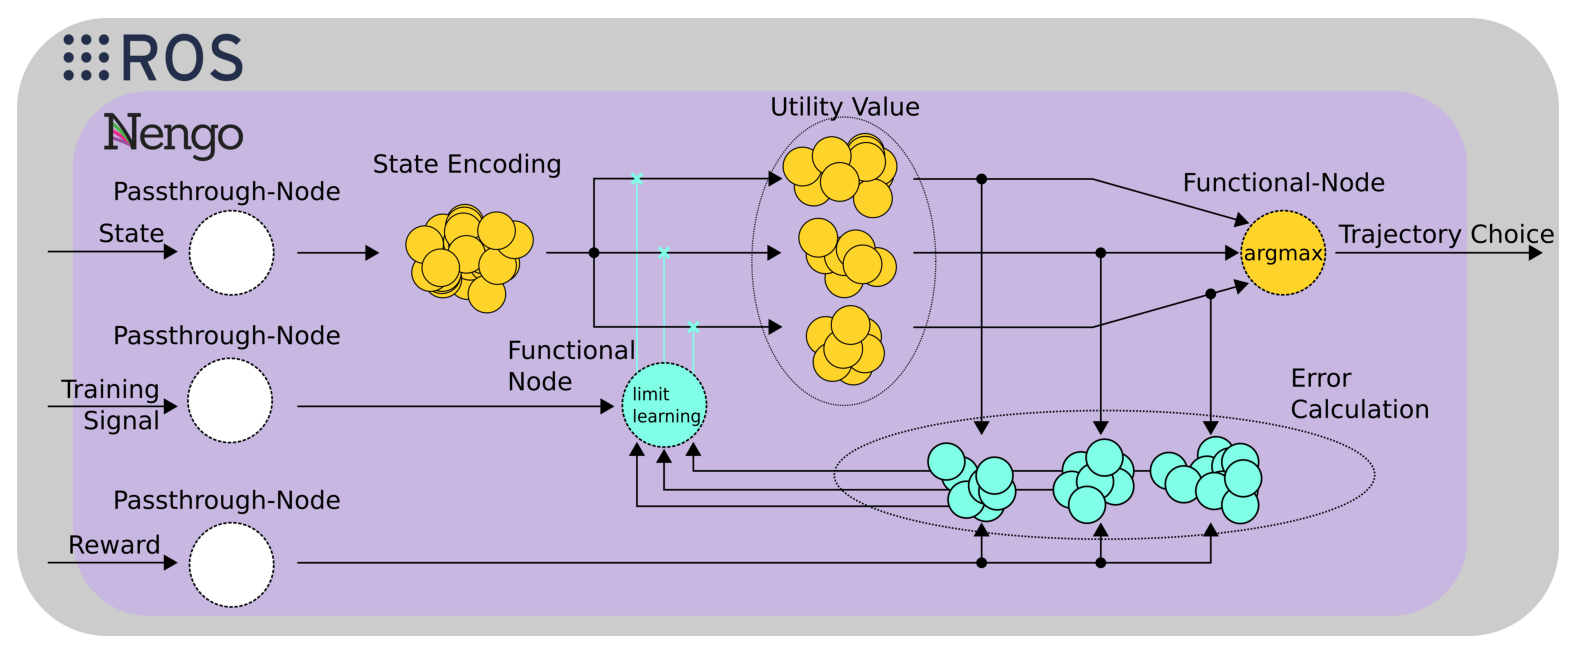
\includegraphics[width=0.65\textwidth]{imgs/SNN.eps}}
% \resizebox{0.65\textwidth}{!}{\input{imgs/SNN.eps_tex}}}
\hfill
\subfloat[Visualization of a set of exemplary trajectories.\label{fig:trajectories}]{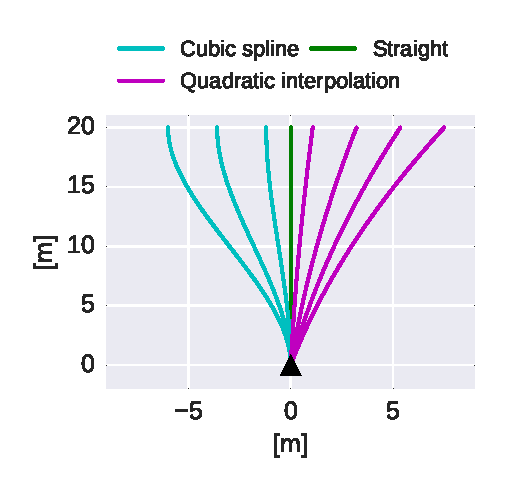
\includegraphics[width=0.3\textwidth]{imgs/trajectories.eps}}
\caption{\ac{SNN} for \emph{trajectory selection} and exemplary set of trajectories}
\end{figure}

\subsubsection{Trajectory selection module}%
\label{ssubsec:trajectory_selection_module}

We focus on the \emph{trajectory selection} module isolated from the other modules.
Therefore, we use a classical controller to steer the vehicle along the chosen trajectories at a fixed velocity of \SI{34}{\kilo\metre\per\hour} with the trajectories' end points' longitudinal component set to \SI{20}{\metre} which emulates a simplified version of \emph{trajectory following}. \par
We implemented a set of \num{15} trajectories to describe varying degrees of different behaviors (see Fig. \ref{fig:trajectories}).
We use straight lines to emulate lane following, cubic splines (with their derivative set to \num{0} at the extremities) to model lane change maneuvers and quadratic interpolations between a start and end point to perform a change in orientation.
The latter trajectories are intended for driving curves or to correct slight misalignments between the vehicle and the road.

\subsection{Reinforcement Learning}%
\label{subsec:reinforcement_learning_network}

The core of this work is the learning \acl{SNN} for \emph{trajectory selection}, which  is visualized in Fig. \ref{fig:snn} and consists of two sub-networks.
It was built using the Nengo neural simulator \cite{Bekolay2013}, which implements the principles of the \ac{NEF} \cite{Eliasmith2003}.
The first sub-network $A$ (yellow components in Fig. \ref{fig:snn}) encodes the current state in a neural population.
This population feeds its output to an array of downstream populations, each representing the utility value $Q$ associated to one of the possible actions.
Unless an exploration step is enforced, the highest filtered utility value determines the next action to be performed.
As we want to adapt the mapping between input (state) and utility values by learning the respective connection weights, their decoders are initialized to a fixed value. 
The second sub-network $B$ (cyan components in Fig. \ref{fig:snn}) encodes the reward received from the environment (cf.\ equation \eqref{eq:reward}).
From this reward, the offset to the current utility values is calculated, which in turn is used to adapt the weights of sub-network $A$'s learning connection.

\subsubsection{Learning rule}%
\label{ssubsec:learning_rule}

\begin{figure}[t!]
\centering
\subfloat[Training]{
  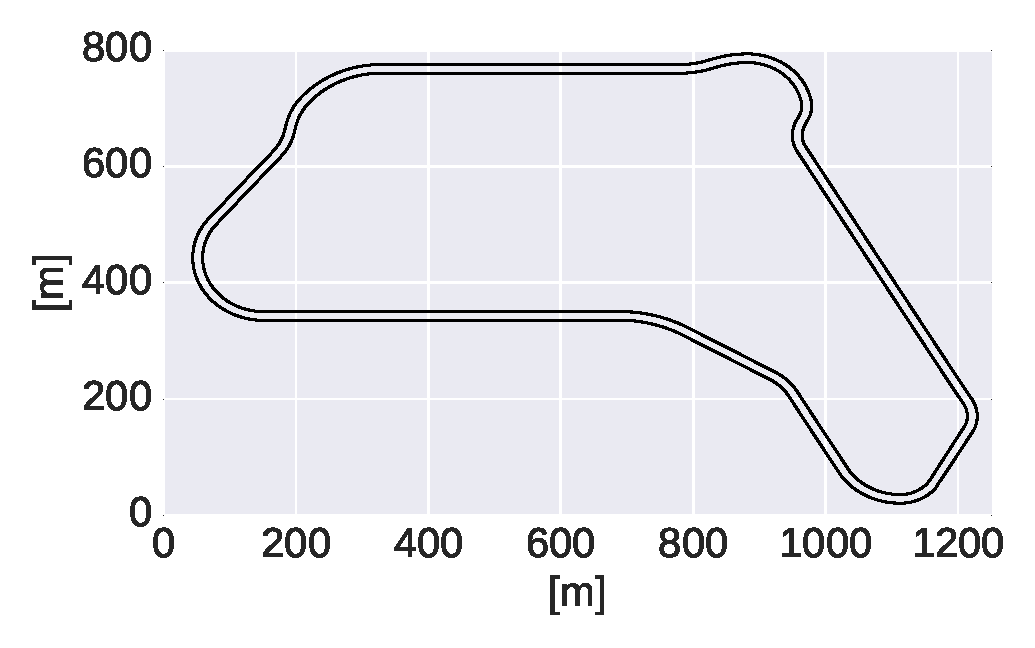
\includegraphics[height=5cm]{imgs/CG2.eps}
}
\hspace{1cm}
\subfloat[Validation]{
  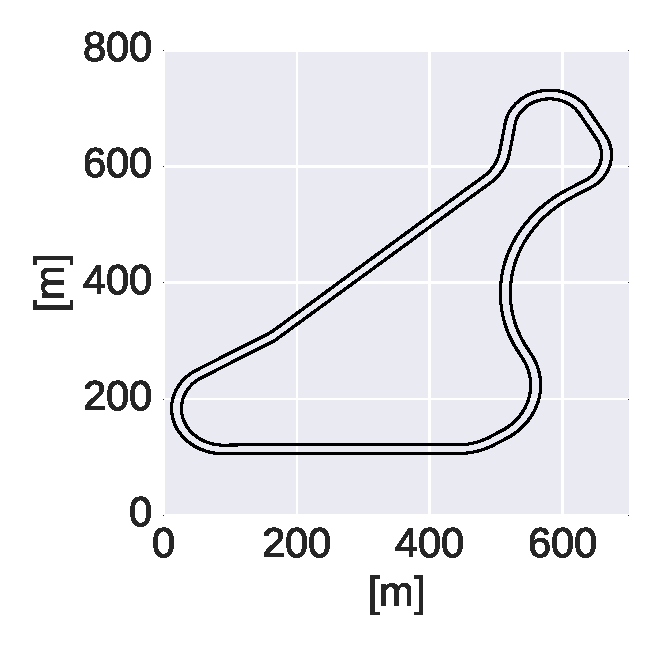
\includegraphics[height=5cm]{imgs/CG1.eps}
}
\caption{Visualization of the chosen training and validation tracks.}
\label{fig:tracks}
\end{figure}
The associative learning process is implemented using the \ac{PES} \cite{Bekolay2013} learning rule, which modifies connection weights based on a (multi-dimensional) error signal $\textbf{e}$.
We calculate the error from the reward function
\begin{align}
r(t) = \lvert p(t) \rvert~\beta_1 \cdot \lvert \theta(t) \rvert ~ \beta_2+ \lvert p(t)-p(t-1) \rvert ~ \beta_3+ \lvert \theta(t)-\theta(t-1) \rvert ~ \beta_4 \text{,}
\label{eq:reward}
\end{align}
where $p$ describes the vehicle's lateral position along the road at successive time steps $t$ and $t-1$ (a value of \num{1} being centered and \num{0} being at the track boundary), $\theta$ describes the vehicle's orientation with respect to the road's centerline (values of \num{1} resp. \num{0} indicate parallel resp.\ perpendicular alignment) and $\beta_k$ being scalar weights.
Thus, the reward function is designed to blend the two objectives of driving aligned with and centered on the road.

With each ensemble representing a utility value $Q(s,a_j)$ of the state $s$  when taking action $a_j$, we define the error for dimension $j$ as

\begin{align}
e_j = \begin{cases}
r(t) - Q(s(t),a_j) & \text{if } a_j \text{ is selected}\\
0 & \text{else}.
\end{cases}
\end{align}

Here, we have chosen to limit the agent's knowledge to immediate rewards.
Therefore, we neglect the correlation between the \emph{trajectory selection} and \emph{time horizon} modules, as it will introduce a temporal component to the discretization.
Hence, the training procedure needs to be adjusted once both modules are trained jointly.
Naturally, such a limited approach will impair the quality of our results.
Our goal, however, is to show general feasibility of our approach which is why we postpone the coupling with other distributed modules to future work.

\subsubsection{Training procedure}%
\label{ssubsec:training_procedure}

In order to evaluate the derived policy's performance, we chose one training and one validation track (Fig. \ref{fig:tracks}) that show similar characteristics in road width and occurring curvatures. They, therefore, show comparable features while being distinct enough to identify if a straight mapping to the training track were to happen.
Whenever the vehicle leaves the track during training, the simulation is reset and a reward of \num{0} is awarded as the track sensors become unreliable in such a scenario.
After every five training runs, three runs until the vehicle goes off-track are driven on the validation course without updating any weights. This process constitutes one training/validation episode.

We use the percentage of completion on the validation track multiplied by the collected average reward in that validation episode as a measure of reliability performance. 
This measure is additionally normalized by the maximally achievable reward for the utilized parameter set.
As the reset leads to a large bias in the experience of states close to the starting line during training, several cyclic points of interests have been defined up-front as substitute starting points before which a non-neuromorphic controller handles the vehicle.
This procedure ensures a large exploration of different possible states and accelerates learning. 
During training, a linearly decaying epsilon exploration is utilized.

\subsubsection{Results}%
\label{ssubsec:results}

\begin{figure}[t!]
\centering
  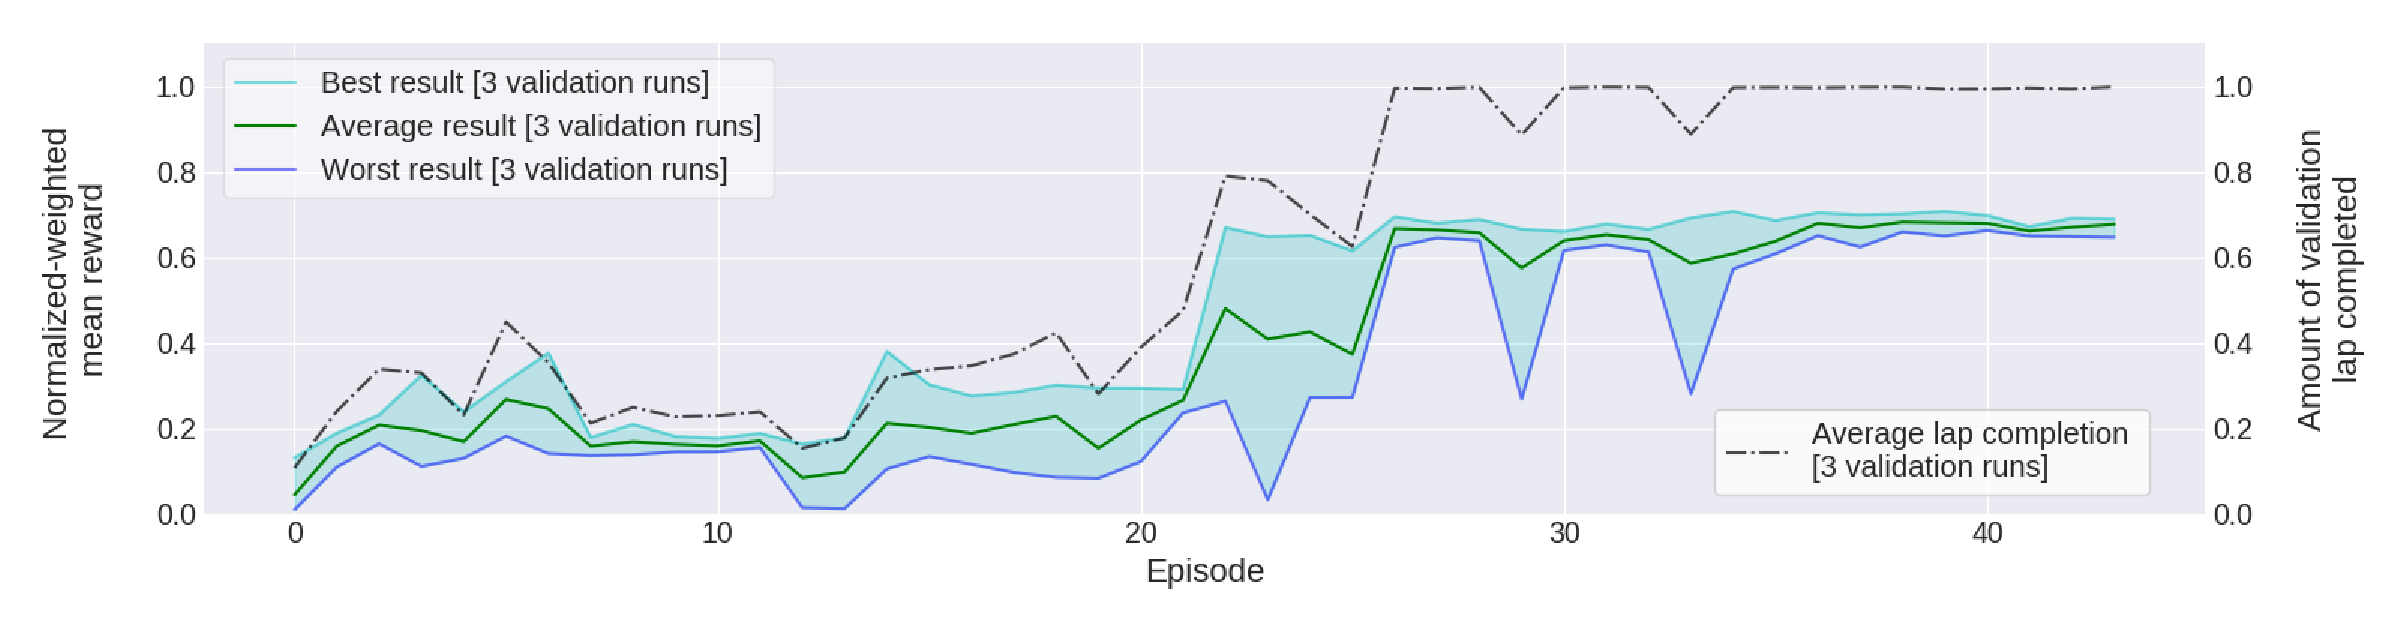
\includegraphics[width=0.95\textwidth]{imgs/CG1-val-updated.eps}
\caption{Results (mean reward and lap completion) for three validation runs per episode \label{fig:results}}
\end{figure}
Fig. \ref{fig:results} visualizes the performance of the derived control policy on the validation track after each episode.
The average performance tends to increase, indicating an overall improvement of the policy given the state values approximated by the \ac{SNN}.
The neuromorphic controller is able to reliably complete the validation lap after roughly \num{35} episodes without having performed any training on it.
This indicates that the \ac{SNN} is able to learn a meaningful policy and to generalize beyond the training track given the sensors' uncertainties.

\subsection{Summary}%
\label{subsec:summary_vehicle_control}

Our investigation in this section shows promise to be a first step in the direction of a neuromorphic vehicle control.
Although we chose a very limited approach in associative reinforcement learning, our system is able to fulfill the initial requirement to complete laps on the unknown validation track.
However, tests on other validation tracks revealed issues with this approach.
Successive curves are a problematic situation as the vehicle manages to pass the first curve but oftentimes maneuvers itself into a position where it is impossible to complete the second curve with the available trajectories.
This problem can not be identified timely, and therefore solved with the current approach, as there is no temporal component in associative reinforcement learning. 

\subsubsection{Outlook}%
\label{ssubsec:outlook}

We envision to tackle the temporal issue using Q-learning with \textit{dual learning}.
Another direction for future work is to couple the \emph{trajectory selection} with the \emph{time horizon} module to enable planning over time while remaining within a discretized domain and delaying the continuous control to the \emph{trajectory following} module.
These modules could be trained separately or jointly to evaluate applicability of this more sophisticated approach.


\section{Summary}%
\label{sec:summary_closed_loop_systems}

In this chapter, we have presented a first step towards a neuromorphic control architecture.
Due to the absence of a suitable vehicle demonstrator, lacking integration of neuromorphic prototypes into current vehicle hardware architectures and finally due to safety considerations, we have demonstrated the general feasibility of such a neuromorphic control architecture in two sample instantiation.
First, we presented a proof-of-concept implementation of a non-trivial mobile robot manipulation tasks in the substrate of \acp{SNN}.
We showed, that our architecture can be used to induce human expert knowledge into neural task implementations.
Such manually designed networks can either be used to complement other, decoupled learning networks or serve as a basis to bootstrap learning to avoid starting the training procedure from a completely blank state.
The second proof-of-concept implementation combines manual designed and automatically learned networks in the context of short-term vehicle trajectory planning.
We use reinforcement learning in \acp{SNN} to select trajectories for a classical controller, which is decoupled from the learning network.
Thereby, we demonstrate that neuromorphic principles can be used in the context of vehicle control.
However, today's vehicle architectures are not designed yet to integrate neuromorphic hardware, which on the other hand have not reached the technical and commercial maturity to be integrated in such architectures.
This lack of integration prohibits the adoption of any algorithm implemented in a spiking neuron substrate into vehicle applications, since the advantages of this algorithmic substrate are closely coupled to energy-efficient deployment on dedicated hardware.
That is, one of the unique strengths of \acp{SNN} in contrast to more traditional learning approaches is their ability to be efficiently processed on neuromorphic hardware mostly leading to a trade-off between efficiency and higher accuracy delivered by traditional approaches.


